\part{新约}


\chapter*{新约全书导论}
\addcontentsline{toc}{chapter}{新约全书导论}
“新约全书”是\UL[耶稣]死后,由其宗徒弟子,在天主圣神的默感与引导之下,所写成的经典汇集。此汇集由第二世纪起即称为《新约书》,或简称《新约》。称之为“约”,因为其中所讲论的,是天主与人类所立的盟约;称之为“新”,以别于“旧约”。“旧约”是天主与\UL[以]民在\UL[西乃]山上所立的圣约,而“新约”是\UL[基督]以自己的圣血与圣死,在天主与人间,所建立的救恩圣约(参阅\uwave{玛}26:28;\uwave{谷}14:24等处)。

“新约全书”,按圣教会古老的传授,共计二十七卷;

《历史书》五卷:《玛窦福音》、《马尔谷福音》、《路加福音》、《若望福音》和《宗徒大事录》。

《训诲书》二十一卷:圣\UL[保禄]快十四封:《罗马书》、《格林多》前后二书、《迦拉达书》、《厄弗所书》、《斐理伯书》、《哥罗森书》、《得撒洛尼》前后二书、《弟茂德》前后二书、《弟铎书》、《费肋孟书》和《希伯来书》;公函七封:《雅各伯书》、《伯多禄》前后二书、《若望》一、二、三书并《犹达书》。

《先知书》一卷:《若望默示录》。

《新约全书》,除《玛窦福音》的原文为\UL[阿刺美]文外,都是用\UL[希腊]文写成的。这些似乎有些奇怪,因为按当时\UL[耶稣]在世时,和宗徒最初讲道时所用的语言,本来都是\UL[阿刺美]语,并且全部《新约》作者,除圣\UL[路加]外,又都是\UL[犹太]人;那么为什么不用本国文字编写呢?其理由是因为只有《玛窦福音》是写给\UL[巴力斯坦]的\UL[犹太]人,而其余的书都是写给说\UL[希腊]话的基督徒,其中很少有通晓\UL[阿刺美]语的;更何况《新约》又是向天下万民所公布的;因此以当时\UL[罗马]帝国内所通行的\UL[希腊]语编写,是很自然的事。

《新约全书》(或《新经》),就宗教方面来说,远远超过《旧约全书》(或《古经》),因为天主在旧约时代只是“多次并以多种方式,藉着先知对祖先说过话”;然而在新约时代却是“藉着了对我们说了话”(\uwave{希}1:1)。如此,旧约的启示在新约内才得以圆满;旧约的预许在新约内才得以实现。所以吾人除非认识《新约》,决不能完全明了《旧约》;为此,可说《新约全书》实是世界上最重要和最宝贵的作品。


\chapter*{福音总论}
\addcontentsline{toc}{chapter}{福音总论}
“福音”一词,按其字音,原指“喜讯”;但按《新约》作者彩此词的意义来说,乃是指天主子\UL[耶稣]隆重为人,从天上给人类带来的启示,和在他完成救赎工程以后,诸宗徒向万民所宣布的得救喜讯。

这喜讯的传报,最初只靠口头的宣讲,稍后才有不少人士把\UL[耶稣]的生平与宣讲笔之于书,因而产生了“福音”的著作。按\uwave{路}1:1的记载,这样的著作在当时已为数不少,可是圣教会自初只承认《玛窦》、《马尔谷》、《路加》、《若望》这四部《福音》为受默感而写的经典,并著录在正经书目内,其他名为“福音”的著作,概著录为伪经。

“福音”书虽有四部,但所传述的“福音”却只是一个,因为四圣史所撰述的是同一的喜讯,只是在所采用形式上有所不同而已。前三部《福音》,无论是在取材和结构上,或在用字上,大致可以说相同,甚至可并列对照,一望而知彼此间所有的关系,因而有“对观福音”之称。这三部《福音》之所以如此相同,是因为前三圣史记述了大体相同的“宗徒教理讲授”:\UL[玛窦]记述了\UL[耶路撒冷]教会的传授,\UL[马尔谷]记述了\UL[罗马]教会的传授,\UL[路加]记述了\UL[安提约基雅]教会的传授。\UL[若望]因见前三《福音》已流传于世,没有重述的必要,遂由自己记忆所及,采取了一些有关的材料,在第一世纪末叶,针对当时人事环境的需要,编著了自己的《福音》,其目的是在攻击方兴的异端邪说。

四《福音》虽然不是狭义的史书,但就信实性来说:世界上没有一部史书可与之相比,因为各位作者,或是目睹所述之事的宗徒(\UL[玛窦]、\UL[若望]),或是宗徒的亲传弟子(\UL[马尔谷]、\UL[路加]),他们所依据的,全是亲历其事人物的口述;况且《福音》成书时,尚有不少耳闻目睹的证人生存于世。

四《福音》内不但包含了有关信仰绝对重要的道理,而且也给世人提示了诸德的完美模范,基督徒成全的最高理想:即为我们降生成人的天主圣子。


\chapter*{玛窦福音引言}
\addcontentsline{toc}{chapter}{玛窦福音引言}
第一部《福音》的作者是圣\UL[玛窦]宗徒。\UL[玛窦]又名\UL[肋未],是\UL[阿耳斐]的儿子(\uwave{谷}2:14)。他在\UL[耶稣]召叫之前,曾在\UL[葛法翁]作过税吏。他一被召,即刻舍弃一切,跟随了\UL[耶稣](\uwave{玛}9:9;\uwave{谷}2:13、14;\uwave{路}5:27、28)。\UL[耶稣]升天后,他先在\UL[巴力斯坦]一带,给自己的同胞宣讲福音多年,然后动身往外方传教去了。最后死在何处何时,史无确证。圣教会从古以来,即认他为一位为主殉道的宗徒,每年九月二十一日庆祝他的瞻礼。

据最古的传授,圣教会始终认为圣\UL[玛窦]是第一部《福音》的作者;这也可由《福音》书内的暗示得到证明:例如\UL[马尔谷]与\UL[路加]记载十二位宗徒名单时,只记了\UL[玛窦]的名字,然而在第一部《福音》内,于“\UL[玛窦]”名字前却加上了受人歧视的“税吏”头衔,可知原作者对自己的职位,毫不避讳。

《玛窦福音》的原著为\UL[阿刺美]文,因为是为\UL[巴力斯坦]的\UL[犹太]人写的,这是自古以来圣教会一致公认的事。此书后来不知由何人译为\UL[希腊]文。本《福音》因为是写给归化的\UL[犹太]人,因此特别为证明\UL[耶稣]\UL[基督]即是天主所预许及先知所预言的“默西亚”。虽然大多数\UL[犹太]人否认\UL[耶稣]为默西亚,并把他置于死地:然而他却由死者中光荣复活,并建立了自己的教会作为天国在世上的开端,继续他救世的使命。由于这个特殊的目的,\UL[玛窦]比其他三位圣史,更强调先知们的预言在\UL[耶稣]身上全应验了。

本书的著作地点,大概是\UL[耶路撒冷]。至于著作时期,原文可说是写于其他《福音》之前,大约著于公元50年左右;现行的\UL[希腊]译本,大概是成于《马尔谷》和《路加》两福音之后,约在公元70年左右。

本书记述\UL[耶稣]言行,并未全按编年的次第,而是出于作者的匠心独运。他把\UL[耶稣]公开传教的整个生活分作五段,每段先记事,后记言。此五段即是:(一)3-7;(二)8-10;(三)11-13:53;(四)13:54-18;(五)19-25。

本《福音》因是四《福音》中材料最丰富的一部,在结构上又是最有系统的一部,为此本《福音》在教会内应用最广,引用最多。


\chapter{玛窦福音}


\section{耶稣童年史(1,2)}


\subsection{第一章 族谱}
$^{1}$\UL[亚巴郎]之子,\UL[达味]之子\UL[耶稣]\UL[基督]的族谱:\textcircled{1}\NoLabelFootnote{1 \textcircled{1}圣史于卷首列出\UL[耶稣]的族谱,是证明救主应生于\UL[亚巴郎]和\UL[达味]后裔的预言,在耶稣向上应验了。“耶稣”意即“救主”(21节),是天主子降生为人的名字。“基督”为\UL[希腊]文,\UL[希伯来]作“默西亚”,意即“受傅者”,表示他的职位和使命。此处族谱如与\uwave{路}3:23-38对照,显然不全。\uwave{玛}仅列举著名者;又为便于记忆,分为三组,每组十四位。}$^{2}$\UL[亚巴郎]生\UL[依撒格],\UL[依撒格]生\UL[雅各伯],\UL[雅各伯]生\UL[犹大]和他的兄弟们;$^{3}$\UL[犹大]由\UL[塔玛尔]生\UL[培勒兹]和\UL[则辣黑],\UL[培勒兹]生\UL[赫兹龙],\UL[赫兹龙]生\UL[阿兰]。$^{4}$\UL[阿兰]生\UL[阿米纳达布],\UL[阿米纳达布]生\UL[纳赫雄],\UL[纳赫雄]生\UL[撒耳孟],$^{5}$\UL[撒耳孟]由\UL[辣哈布]生\UL[波阿次],\UL[波阿次]由\UL[卢德]生\UL[敖贝得],\UL[傲贝得]生\UL[叶瑟],$^{6}$\UL[叶瑟]生\UL[达味王]。\UL[达味]由\UL[乌黎雅]的妻子生\UL[撒罗满],$^{7}$\UL[撒罗满]生\UL[勒哈贝罕],\UL[勒哈贝罕]生\UL[阿彼雅],\UL[阿彼雅]生\UL[阿撒],$^{8}$\UL[阿撒]生\UL[约沙法特],\UL[约沙法特]生\UL[约兰],\UL[约兰]生\UL[乌齐雅],$^{9}$\UL[乌齐雅]生\UL[约堂],\UL[约堂]生\UL[阿哈次],\UL[阿哈次]生\UL[希则克雅]。$^{10}$\UL[希则克雅]生\UL[默纳舍],\UL[默纳舍]生\UL[阿孟],\UL[阿孟]生\UL[约史雅],$^{11}$\UL[约史雅]在\UL[巴比伦]流徙期间生\UL[耶苛尼雅]和他的兄弟们。$^{12}$流徙\UL[巴比伦]以后,\UL[耶苛尼雅]生\UL[沙耳提耳],\UL[沙耳提耳]生\UL[则鲁巴贝耳],$^{13}$\UL[则鲁巴贝耳]生\UL[阿彼乌得],\UL[阿彼乌得]生\UL[厄里雅金],\UL[厄里雅金]生\UL[阿左尔]。$^{14}$\UL[阿左尔]生\UL[匝多克],\UL[匝多克]生\UL[阿歆],\UL[阿歆]生\UL[厄里乌得],$^{15}$\UL[厄里乌得]生\UL[厄肋阿匝尔],\UL[厄肋阿匝尔]生\UL[玛堂],\UL[玛堂]生\UL[雅各伯],$^{16}$\UL[雅各伯]生\UL[若瑟],\UL[玛利亚]的丈夫,\UL[玛利亚]生\UL[耶稣],他称为\UL[基督]。\textcircled{2}\NoLabelFootnote{1 \textcircled{2}\UL[玛利亚]因圣神的德能受孕生耶稣(20节;\uwave{路}1:35),为此族谱中未说:\UL[若瑟]生耶稣;但\UL[若瑟]在名义和法律上仍是\UL[耶稣]的父亲,有为父的一切权利(21,25两节)。}$^{17}$所以从\UL[亚巴郎]到\UL[达味]共十四代,从\UL[达味]到流徙\UL[巴比伦]共十四代,从流{徙}\UL[巴比伦]到\UL[基督]共十四代。


\subsubsection{生于童贞女}
$^{18}$\UL[耶稣]\UL[基督]的诞生是这样的:他的母亲\UL[玛利亚]许配于\UL[若瑟]后,在同居前,她因圣神有孕的事已显示出来。$^{19}$她的丈夫\UL[若瑟],因是义人,不愿公开羞辱她,有意暗暗地休退她。$^{20}$当他在思虑这事时,看,在梦中上主的天使显现给他说:“\UL[达味]之子\UL[若瑟],不要怕娶你的妻子\UL[玛利亚],因为那在她内受生的,是出于圣神。$^{21}$她要生一个儿子,你要给他起名叫\UL[耶稣],因为他要把自己的民族,由他们的罪恶中拯救出来。“$^{22}$这一切事的发生,是为应验上主籍先知所说的话。$^{23}$”看,一位贞女,将怀孕生子,人将称他的名字为\UL[厄玛奴耳],意思是:天主与我们同在。\textcircled{3}\NoLabelFootnote{1 \textcircled{3}\uwave{依}7:14。}$^{24}$\UL[若瑟]从睡梦中醒来,就照上主的天使所嘱咐的办了,娶了他的妻子;$^{25}$\UL[若瑟]虽然没有认识她,她就生了一个儿子,给他起名叫\UL[耶稣]。


\subsection{第二章 贤士来朝}
$^{1}$当\UL[黑落德]为王时,\UL[耶稣]诞生在\UL[犹大]的\UL[白冷];看,有贤士从东方来到\UL[耶路撒冷],\textcircled{1}\NoLabelFootnote{2 \textcircled{1}贤士是当时中东一带热心宗教和观察星宿的人。前来朝拜救主的外方贤士,显然熟知\UL[巴郎]的预言 (\uwave{户}24:17)。贤士为三位和为王的传说,似乎来自\uwave{依}60:1-6;\uwave{咏}72:10、11的预言和所献的三样礼物。}$^{2}$说:“才诞生的\UL[犹太]人君王在哪里?我们在东方见到了他的星,特来朝拜他。”$^{3}$\UL[黑落德]王一听说,就惊慌起来,全\UL[耶路撒冷]也同他一起惊慌。\textcircled{2}\NoLabelFootnote{2 \textcircled{2}\UL[耶路撒冷]所以惊慌,是因为怕:暴君\UL[大黑落德]因怕新君夺他的王位,又要屠杀人民。}$^{4}$他便召集了众司祭长和民间的经师,仔细考问他们:\UL[默西亚]应当生在哪里。$^{5}$他们对他说:“在\UL[犹大]的\UL[白冷],因为先知曾这样记载:$^{6}$‘你\UL[犹大]地\UL[白冷]啊!你在\UL[犹大]的郡邑中,决不是最小的,因为将由你出来一位领袖,他将牧养我的百姓\UL[以色列]。’”\textcircled{3}\NoLabelFootnote{2 \textcircled{3}\uwave{米}5:1-3。}$^{7}$于是\UL[黑落德]暗暗把贤士叫来,仔细询问他们那星出现的时间;$^{8}$然后打发他们往\UL[白冷]去,说:“你们去仔细寻访婴孩,几时找到了,给我报信,好让我也去朝拜他。”$^{9}$他们听了王的话,就走了。看,他们在东方所见的那星,走在他们前面,直至来到婴孩所在的地方,就停在上面。$^{10}$他们一见到那星,极其高兴欢喜。$^{11}$他们走进屋内,看见婴儿和他的母亲\UL[玛利亚],遂俯伏朝拜了他,打开自己的宝匣,给他奉献了礼物,即黄金、乳香和没药。$^{12}$他们在梦中得到指示,不要回到\UL[黑落德]那里,就由另一条路返回自己的地方去了。


\subsubsection{圣家逃往埃及}
$^{13}$他们离去后,看,上主的天使托梦显于\UL[若瑟]说:“起来,带着婴孩和他的母亲逃往\UL[埃及]去,住在那里,直到我再通知你,因为\UL[黑落德]即将寻找这婴孩,要把他杀掉。”$^{14}$\UL[若瑟]便起来,星夜带了婴孩和他的母亲,退避到\UL[埃及]去了。$^{15}$留在那里,直到\UL[黑落德]死去。这就应验了上主藉先知所说的话:“我从\UL[埃及]召回了我的儿子。”\textcircled{4}\NoLabelFootnote{2 \textcircled{4}\uwave{欧}11:1。圣史以天主领\UL[以]民出\UL[埃及],作为天主领\UL[耶稣]出\UL[埃及]的预象。}


\subsubsection{无罪婴孩遭屠杀}
$^{16}$那时,\UL[黑落德]见自己受了贤士们的愚弄,就大发忿怒,依照他由贤士们所探得的时期,差人将\UL[白冷]及其周围境内所有两岁及两岁以下的婴儿杀死。$^{17}$于是应验了\UL[耶肋米亚]先知所说的话:$^{18}$“在\UL[辣玛]听到了声音,痛哭哀号不止;\UL[辣黑耳]痛哭他的子女,不愿受人的安慰,因为他们不在了。”\textcircled{5}\NoLabelFootnote{2 \textcircled{5}圣史借用了\uwave{耶}31:15,以哀哭\UL[以]民充军的先祖母\UL[辣黑耳],作为\UL[白冷]丧子者的预像,因\UL[辣黑耳]的坟墓靠近\UL[白冷]。}


\subsubsection{圣家回国}
$^{19}$\UL[黑落德]死后,看,上主的天使在\UL[埃及]托梦显于\UL[若瑟],$^{20}$说:“起来,带着孩子和他的母亲,往\UL[以色列]地去,因为那些谋杀孩子性命的人死了。”$^{21}$他便起来,带了孩子和他的母亲,进了\UL[以色列]地域;$^{22}$但是一听说\UL[阿尔赫劳]继他父亲\UL[黑落德]作了\UL[犹太]王,就害怕到那里去;梦中得了指示后,便退避到\UL[加里肋亚]境内,\textcircled{6}\NoLabelFootnote{2 \textcircled{6}\UL[大黑落德]王卒于公元前四年,由\UL[阿尔赫劳]继位。此人生性好杀,为此\UL[若瑟]“害怕到那里去”。那时,管理\UL[加里肋亚]省的\UL[黑落德]\UL[安提帕]不似前者凶残。}$^{23}$去住在一座名叫\UL[纳匝肋]的城中,如此应验了先知们所说的话:“他将称为\UL[纳匝肋]人。”\textcircled{7}\NoLabelFootnote{2 \textcircled{7}此语辞句虽不见于《旧约》,但按\UL[耶稣]被轻视的事,实已应验了先知的预言(\uwave{依}53)。\UL[纳匝肋]也是当时被轻视的地方(\uwave{若}1:46)。}


\section{耶稣传教史 宣布天国的福音}


\subsection{第三章 若翰讲道施洗}
$^{1}$那时,洗者\UL[若翰]出现在\UL[犹太]旷野宣讲,$^{2}$说:“你们悔改吧!因为天国临近了。”$^{3}$这人便是那藉\UL[依撒意亚]先知所预言的:“在旷野里有呼号者的声音:你们该当预备上主的道路,修直他的途径。”\textcircled{1}\NoLabelFootnote{3 \textcircled{1}\uwave{依}40:3。所说“天国”(\uwave{谷}、\uwave{路}称“天主的国”),即先知所预言\UL[默西亚]要立的神国(\uwave{达}7:13-17)。称为“天国”或“天主的国”,因为它的来源、组织、道理、法律和目的,都是由天主而来或属于天上的;也称为“基督的国”(\uwave{弗}5:5;\uwave{哥}1:13);因为是\UL[耶稣]所宣讲和建立的。}$^{4}$这\UL[若翰]穿着骆驼毛做的衣服,腰间束着皮带,他的食物是蝗虫和野蜜。$^{5}$那里,\UL[耶路撒冷]、全\UL[犹太]以及全\UL[约旦]河一带的人,都出来到他那里去,$^{6}$承认自己的罪过,并在\UL[约但]河里受他的洗。\textcircled{2}\NoLabelFootnote{3 \textcircled{2}\UL[若翰]所行的是悔罪的洗礼,使人改恶迁善,准备迎接天国的来临,与\UL[耶稣]所立赦罪的洗礼全然不同。}$^{7}$他见到许多\UL[法利塞]人和\UL[撒杜塞]人来受他的洗,就对他们说:“毒蛇的种类!谁指教你们逃避那即将来临的忿怒?$^{8}$那么,就结与悔改相称的果实吧!$^{9}$你们自己不要思念说:我们有\UL[亚巴郎]为父。我给你们说:天主能从这些石头给\UL[亚巴郎]兴起子孙来。$^{10}$斧子已放在树根上了,凡不结好果子的树,必被砍倒,投入火中。$^{11}$我固然用水洗你们,为使你们悔改;但在我以后要来的那一位,比我更强,我连提他的鞋也不配,他要以圣神及火洗你们。$^{12}$他的簸箕已在他手中,他要扬净自己的禾场,将他的麦粒收入仓内。至于糠秕,却要用不灭的火焚烧。”\textcircled{3}\NoLabelFootnote{3 \textcircled{3}\UL[若翰]的严辞斥责是针对\UL[法利塞]和\UL[撒杜塞]两党人:前者多顾形式,以为谨守法律即可成义人;后者不信死后复活的道理,为此他们都不怕未来的审判。\UL[若翰]却说要来的默西亚必认真审判世人的善恶真伪(\uwave{路}3:1-18)。}


\subsubsection{耶稣受洗}
$^{13}$那时,\UL[耶稣]由\UL[加里肋亚]来到\UL[约但]河\UL[若翰]那里,为受他的洗;$^{14}$但\UL[若翰]想要阻止他说:“我本来需要受你的洗。而你却来就我吗?”$^{15}$\UL[耶稣]回答他说:“你暂且容许吧!因为我们应当这样,以完成全义。”于是\UL[若翰]就容许了他。\textcircled{4}\NoLabelFootnote{3 \textcircled{4}“完成全义”,即谓天主愿意默西亚满全一切法律,作为齐全圣善的模范。此洗礼既为圣善的事,他就不应例外。}$^{16}$\UL[耶稣]受洗后,立时从水里上来,忽然天为他开了。他看见天主圣神有如鸽子降下,来到他上面;$^{17}$又有声音由天上说:“这是我的爱子,我所喜悦的。”\textcircled{5}\NoLabelFootnote{3 \textcircled{5}三位一体的天主,每位在这隆重的仪式中都显示于外,参加救赎工程的开幕大典。}


\subsection{第四章 耶稣禁食三退魔诱}
$^{1}$那时,\UL[耶稣]被圣神领往旷野,为受魔鬼的试探。$^{2}$他四十天四十夜禁食,后来就饿了。$^{3}$试探者就前来对他说:“你若是天主子,就命这些石头变成饼吧!”$^{4}$他回答说:“经上记载:‘人生活不只靠饼,而也靠天主口中所发的一切言语。’”\textcircled{1}\NoLabelFootnote{4 \textcircled{1}\uwave{申}8:3}$^{5}$那时,魔鬼引他到了圣城,把他立在殿顶上,$^{6}$对他说:“你若是天主子,就跳下去,因经上记载:‘他为你吩咐了自己的天使,他们要用手托着你,免得你的脚碰在石头上。’”\textcircled{2}\NoLabelFootnote{4 \textcircled{2}\uwave{咏}91:11、12。}$^{7}$\UL[耶稣]对他说:“经上又记载:‘你不可试探上主,你的天主!’”\textcircled{3}\NoLabelFootnote{4 \textcircled{3}\uwave{申}6:16。}$^{8}$魔鬼又把他带到一座极高的山上,将世上的一切国家及其荣华指给他看,$^{9}$对他说:“你若俯伏朝拜我,我必把这一切交给你。”$^{10}$那时,\UL[耶稣]就对他说:“去吧!撒殚!因为经上记载:‘你要朝拜上主,你的天主,惟独事奉他。’”\textcircled{4}\NoLabelFootnote{4 \textcircled{4}\uwave{申}6:13。魔鬼试探\UL[耶稣]的目的,是要他迎合\UL[犹太]人对默西亚建立富强国家的妄想,而放弃以苦难死亡作救赎的代价。但是耶稣没有迎合此种妄想,拒绝了魔鬼的诱惑,给人留下了退诱惑的榜样。}$^{11}$于是魔鬼离开了他,就有天使前来伺候他。


\subsubsection{在加里肋亚开始传道}
$^{12}$\UL[耶稣]听到\UL[若翰]被监禁以后,就退避到\UL[加里肋亚]去了;$^{13}$后又离开\UL[纳匝肋],来住在海边的\UL[葛法翁],即住在\UL[则步隆]和\UL[纳斐塔里]境内。$^{14}$这应验了\UL[依撒意亚]先知所说的话:$^{15}$\UL[则步隆]地与\UL[纳斐塔里]地,通海大路,\UL[约但]河东,外方人的\UL[加里肋亚],$^{16}$那坐在黑暗中的百姓,看见了浩光;那些坐在死亡阴影之地的人,为他们出现了光明。“$^{17}$从那时起,\UL[耶稣]开始宣讲说:”你们悔改吧!因为天国临近了。“\textcircled{5}\NoLabelFootnote{4 \textcircled{5}\UL[加里肋亚]地方自公元前八世纪\UL[以色列]国灭亡后,历来为外邦人徙居之地。耶稣却在此地宣讲福音,使那些居于黑暗的人见了光明,因此应验了\uwave{依}8:23等处对此事的预言。}


\subsubsection{召收首批门徒}
$^{18}$\UL[耶稣]沿\UL[加里肋亚]海行走时,看见了两个兄弟:称为\UL[伯多禄]的\UL[西满],和他的兄弟\UL[安德肋],在海里撒网,他们原是渔夫。$^{19}$他就对他们说:”来,跟从我!我要使你们成为渔人的渔夫。“$^{20}$他们立刻舍下网,跟随了他。$^{21}$他从那里再往前行,看见了另外两个兄弟:\UL[载伯德]的儿子\UL[雅各伯]和他的弟弟\UL[若望],在船上同自己的父亲\UL[载伯德]修理他们的网,就召叫了他们。$^{22}$他们也立刻舍下鱼船和自己的父亲,跟随了他。


\subsubsection{在加里肋亚开始显奇迹}
$^{23}$\UL[耶稣]走遍了全\UL[加里肋亚],在他们的会堂内施教,宣讲天国的福音,治好民间各种疾病,各种灾殃。$^{24}$他的名声传遍了整个\UL[叙利亚]。人就把一切有病的,受各种疾病痛苦煎熬的、附魔的、癫痫的、瘫痪的,都给他送来,他都治好了他们。$^{25}$于是有许多群众从\UL[加里肋亚]、”十城区“、\UL[耶路撒冷]、\UL[犹太]和\UL[约但]河东岸来跟随了他。\textcircled{6}\NoLabelFootnote{4 \textcircled{6}传福音(5-7章),显奇迹,治好各种疾病(8,9两章),是默西亚已来临的迹象和特征(11:4、5)。}


\section{山中圣训}


\subsection{第五章 真福八端}
$^{1}$\UL[耶稣]一见群众,就上了山,坐下;他的门徒上他跟前来,$^{2}$他遂开口教训他们说:\textcircled{1}\NoLabelFootnote{5 \textcircled{1}就如\UL[梅瑟]在\UL[西乃]山上颁布了旧约的法律,\UL[耶稣]也在靠近\UL[葛法翁]的一座山上,立定了新约的法律,并且解释了旧约法律的意义。}

$^{3}$”神贫的人是有福的,因为天国是他们的。

$^{4}$哀恸的人是有福的,因为他们要受安慰。

$^{5}$温良的人是有福的,因为他们要承受土地。

$^{6}$饥渴慕义的人是有福的,因为他们要得到饱饫。

$^{7}$怜悯人的人是有福的,因为他们要受怜悯。

$^{8}$心里洁净的人是有福的,因为他们要看见天主。

$^{9}$缔造和平的人是有福的,因为他们要称为天主的子女。

$^{10}$为义而受迫害的人是有福的,因为天国是他们的。

$^{11}$几时人为了我而辱骂迫害你们,捏造一切坏话毁谤你们,你们是有福的。$^{12}$你们欢喜踊跃吧!因为你们在天上的赏报是丰厚的,因为在你们以前的先知,人也曾这样迫害过他们。“\textcircled{2}\NoLabelFootnote{5 \textcircled{2}此真福八端包含福音的精神,也是天国施政的政纲。}


\subsubsection{基督徒与世界的关系}
$^{13}$”你们是地上的盐,盐若失了味,可用什么使它再咸呢?它再毫无用途,只好抛在外边,任人践踏罢了。$^{14}$你们是世界的光;建在山上的城,是不能隐藏的。$^{15}$人点灯,并不是放在斗底下,而是放在灯台上,照耀屋中所有的人。$^{16}$照样,你们的光也当在人前照耀,好使他们看见你们的善行,光荣你们在天之父。“
\begin{center}
  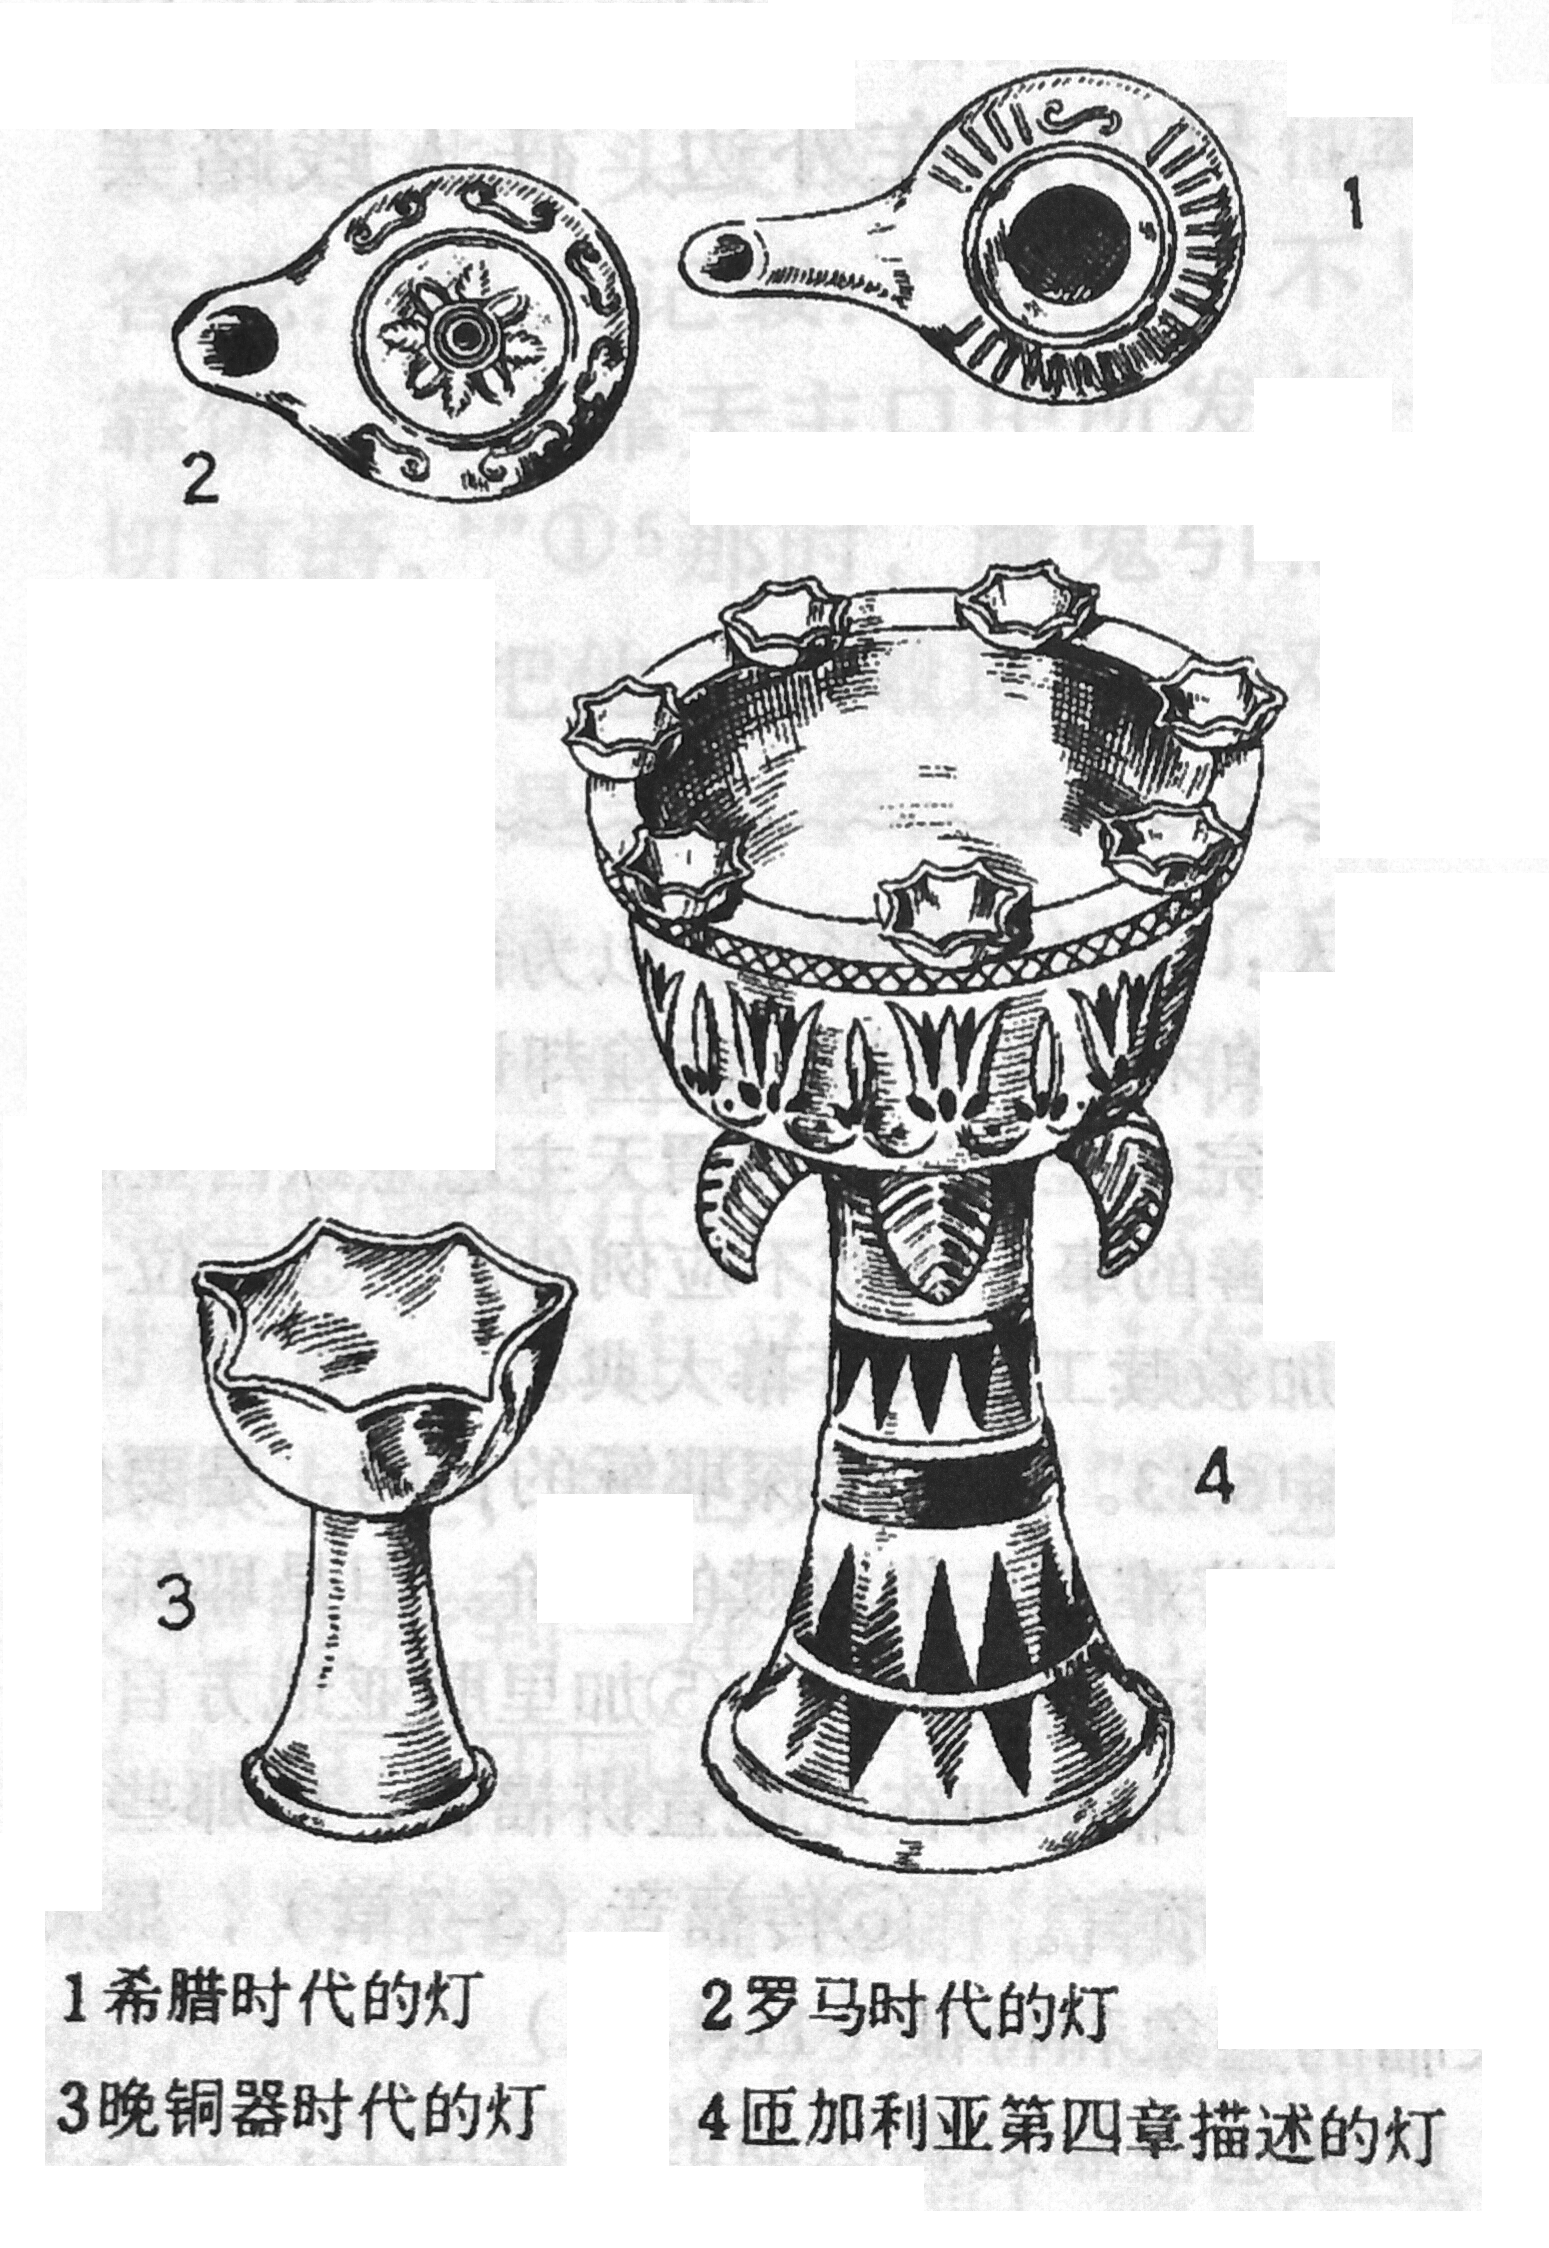
\includegraphics[width=72mm]{images/1514.png}
\end{center}


\subsubsection{新法律成全旧法律}
$^{17}$“你们不要以为我来是废除法律或先知;\textcircled{3}\NoLabelFootnote{5 \textcircled{3}法律与先知即指全部《旧约》。}我来不是为废除,而是为成全。$^{18}$我实在告诉你们:即使天地过去了,一撇或一画也决不会从法律上过去,必待一切完成。$^{19}$所以,谁若废除这些诫命中最小的一条,也这样教训人,在天国里,他将称为最小的;但谁若实行,也这样教训人,这人在天国里将称为大的。$^{20}$我告诉你们:除非你们的义德超过经师和\UL[法利塞]人的义德,你们决进不了天国。\textcircled{4}\NoLabelFootnote{5 \textcircled{4}基督徒的义德,是在于受法律的内外约束,而不是如\UL[法利塞]人所说,只在于法律的外在行为。}

$^{21}$你们一向听过给古人说:“不可杀人!”谁若杀了人,应受裁判。$^{22}$我却对你们说:凡向自己弟兄发怒的,就要受裁判;谁若向自己的弟兄说“傻子”,就要受议会的裁判;谁若说“疯子”,就要受火狱的罚。\textcircled{5}\NoLabelFootnote{5 \textcircled{5}\UL[耶稣]不但禁止人杀人,且也禁止人怀着导引人起杀机的愤怒和辱骂。“疯子”按原文是指不恭敬天主,不守法律的人。“火狱”按原文是指靠近\UL[耶路撒冷]城南烧垃圾和尸体的\UL[革厄纳]山谷(《旧约》常称\UL[本希农])。此山谷作了地狱的象征。}$^{23}$所以,你若在祭坛前,要献你的礼物时,在那里想起你的弟兄有什么怨你的事,$^{24}$就把你的礼物留在那里,留在祭坛前,先去与你的弟兄和好,然后再来献你的礼物。$^{25}$当你和你的对头还在路上,赶快与他和解,免得对头把你交与判官,判官交给差役,把你投在狱里。$^{26}$我实在告诉你:非到你还了最后的一文,决不能从那里出来。

$^{27}$你们一向听说过:“不可奸淫!”$^{28}$我却对你们说:凡注视妇女,有意贪恋她的,他已在心里奸淫了她。$^{29}$若是你的右眼使你跌倒,剜出它来,从你身上扔掉,因为丧失你一个肢体,比你全身投入地狱里,为你更好;$^{30}$若你的右手使你跌倒,砍下它来,从你身上扔掉,因为丧失你一个肢体,比你全身投入地狱里,为你更好。

$^{31}$又说过:“谁若休妻,就该给她休书。”$^{32}$我却给你们说:除了姘居外,凡休自己的妻子的,便是叫她受奸污;并且谁若娶被休的妇人,就是犯奸淫。\textcircled{6}\NoLabelFootnote{5 \textcircled{6}详见19:3-10并注。}

$^{33}$你们又一向听过对古人说:“不可发虚誓!要向上主偿还你的誓愿!”$^{34}$我却对你们说:你们总不可发誓:不可指天,因为天是天主的宝座;$^{35}$不可指地,因为地是他的脚凳;不可指\UL[耶路撒冷],因为她是大王的城市;$^{36}$也不可指你的头发誓,因为你不能使一根头发变白或变黑。$^{37}$你们的话该当是:是就说是,非就说非;其他多余的,便是出于邪恶。\textcircled{7}\NoLabelFootnote{5 \textcircled{7}17-37节,教训人守一切法律。预防犯罪,应由约束内心作起,\UL[法利塞]人即忽略了这一点。}

$^{38}$你们一向听说过:“以眼还眼,以牙还牙。”$^{39}$我却对你们说:不要抵抗恶人;而且,若有人掌击你的右颊,你把另一面也转给他。$^{40}$那愿与你争讼,拿你的内衣的,你连外衣也让给他。$^{41}$若有人强迫你走一千步,你就同他走两千步。$^{42}$求你的,就给他;愿向你借贷的,你不要拒绝。

$^{43}$你们一向听说过:“你应爱你的近人,恨你的仇人!”$^{44}$我却对你们说:你们当爱你们的仇人,当为迫害你们的人祈祷,$^{45}$好使你们成为你们在天之父的子女,因为他使太阳上升,光照恶人,也光照善人;降雨给义人,也给不义的人。$^{46}$你们若只爱那爱你们的人,你们还有什么赏报呢?税吏不是也这样作吗?$^{47}$你们若只问候你们的弟兄,你们作了什么特别的呢?外邦人不是也这样作吗?$^{48}$所以你们应当是成全的,如同你们的天父是成全的一样。”\textcircled{8}\NoLabelFootnote{5 \textcircled{8}基督徒的成全之德是爱,这爱尤其表现于爱仇人。爱仇非出于怯懦,而是效法天父恩待善人也恩待恶人的美德。}


\subsection{第六章 施舍祈祷和禁食的精神}
$^{1}$“你们应当心,不要在人前行你们的仁义,\textcircled{1}\NoLabelFootnote{6 \textcircled{1}“仁义”是泛指施舍、祈祷、禁食等善工。}为叫他们看见;若是这样,你们在天父之前,就没有赏报了。$^{2}$所以,当你施舍时,不可在你前面吹号,如同假善人在会堂及街市上所行的一样,为受人们的称赞;我实在告诉你们,他们已获得了他们他们的赏报。$^{3}$当你施舍时,不要叫你左手知道你右手所行的,$^{4}$好使你的施舍隐而不露,你父在暗中看见,必要报答你。$^{5}$当你祈祷时,不要如同假善人一样,爱在会堂及十字街头立着祈祷,为显示给人;我实在告诉你们,他们已获得了他们的赏报。\textcircled{2}\NoLabelFootnote{6 \textcircled{2}\UL[耶稣]不是指摘公众敬礼,而是指摘不由衷,只图炫耀于人的敬礼。}$^{6}$至于你,当你祈祷时,要进入你的内室,关上门,向你在暗中之父祈祷;你的父在暗中看见,必要报答你。

$^{7}$你们祈祷时,不要唠唠叨叨,如同外邦人一样,因为他们以为只要多言,便可获得垂允。$^{8}$你们不要跟他们一样,因为你们的父,在你们求他以前,已知道你们需要什么。$^{9}$所以,你们应当这样祈祷:

我们在天的父!愿你的名被尊为圣,

$^{10}$愿你的国来临,愿你的旨意承行于地,如在天上一样!

$^{11}$我们的日用粮,求你今天赐给我们;

$^{12}$宽免我们的罪债,犹如我们也宽免得罪我们的人;

$^{13}$不要让我们陷入诱惑,但救我们免于凶恶。\textcircled{3}\NoLabelFootnote{6 \textcircled{3}“天主经”是\UL[耶稣]亲自所传授的最完善的祈祷方式:前段求天主获得光荣,天国成立在世界上,世人承行主旨;后段求个人的日用急需,罪之赦,不为诱惑所陷害。参阅\uwave{路}11:2-4所载“天主经”。}

$^{14}$因为你们若宽免别人的过犯,你们的天父也必宽免你们的;$^{15}$但你们若不宽免别人的,你们的父也必不宽免你们的过犯。$^{16}$几时你们禁食,不要如同假善人一样,面带愁容;因为他们苦丧着脸,是为叫人看出他们禁食来。我实在告诉你们,他们已获得了他们的赏报。$^{17}$至于你,当你禁食时,要用油抹你的头,洗你的脸,$^{18}$不要叫人看出你禁食来,但叫你那在暗中之父看见;你的父在暗中看见,必要报答你。”


\subsubsection{归向天主的纯洁之心}
$^{19}$“你们不要在地上为自己积蓄财宝,因为在地上有虫蛀,有锈蚀,在地上也有贼挖洞偷窃;$^{20}$但该在天上为自己积蓄财宝,因为那里没有虫蛀,没有锈蚀,那里也没有贼挖洞偷窃。$^{21}$因为你的财宝在哪里,你的心也必在哪里。$^{22}$眼睛就是身体的灯。所以,你的眼睛若是康健,你的全身就都光明。$^{23}$但是,如果你的眼睛有了病,你的全身就都黑暗。那么,你身上的光明如果成了黑暗,那该是多么黑暗!”\textcircled{4}\NoLabelFootnote{6 \textcircled{4}以眼喻人心:如人心不为物欲所迷,只想望天上之事,人的生活自然合乎法度;不然,必定是非不分(\uwave{路}11:34-36)。}


\subsubsection{惟独事奉主依恃主的照顾}
$^{24}$“没有人能事奉两个主人:他或是要恨这一个而爱那一个,或是依附这一个而轻忽那一个。你们不能事奉天主而又事奉钱财。

$^{25}$为此,我告诉你们:不要为你们的生命忧虑吃什么,或喝什么;也不要为你们的身体忧虑穿什么。难道生命不是贵于食物,身体不是贵于衣服吗?$^{26}$你们仰观天空的飞鸟,它们不播种,也不收获,也不在粮仓里屯积,你们的天父还是养活它们;你们不比它们更贵重吗?$^{27}$你们中谁能运用思虑,使自己的寿数增加一肘呢?\textcircled{5}\NoLabelFootnote{6 \textcircled{5}“一肘”即言一会儿工夫。此句亦可译作:“使自己的身量增加一肘呢”。}$^{28}$关于衣服,你们又忧虑什么?你们观察一下田间的百合花怎样生长:它们既不劳作,也不纺织;$^{29}$可是我告诉你们:连\UL[撒罗满]在他极盛的荣华时代所披戴的,也不如这些花中的一朵。$^{30}$田地里的野草今天还在,明天就投在炉中,天主尚且这样装饰,信德薄弱的人那,何况你们呢?$^{31}$所以,你们不要忧虑说:我们吃什么,喝什么,穿什么?$^{32}$因为这一切都是外邦人所寻求的;你们的天父原晓得你们需要这一切。$^{33}$你们先该寻求天主的国和它的义德,这一切自会加给你们。$^{34}$所以你们不要为明天忧虑,因为明天有明天的忧虑:一天的苦足够一天受的了。”


\subsection{第七章 各种劝谕}
$^{1}$“你们不要判断人,免得你们受判断,$^{2}$因为你们用什么判断来判断,你们也要受什么判断;你们用什么尺度量给人,也要用什么尺度量给你们。$^{3}$为什么你只看见你兄弟眼中的木屑,而对自己眼中的大梁竟不理会呢?$^{4}$或者,你怎能对你的兄弟说:让我把你眼中的木屑取出来,而你眼中却有一根大梁呢?$^{5}$假善人哪!先从你眼中取出大梁,然后你才看得清楚,取出你兄弟眼中的木屑。

$^{6}$你们不要把圣物给狗,也不要把你们的珠宝投在猪前,怕它们用脚践踏了珠宝,而又转过来咬伤你们。\textcircled{1}\NoLabelFootnote{7 \textcircled{1} 圣物珠宝,指神圣的奥理,狗和猪,指心怀恶意的人。}

$^{7}$你们求,必要给你们;你们找,必要找着;你们敲,必要给你们开,$^{8}$因为凡是求的,就必得到;找的,就必找到;敲的,就必给他开。$^{9}$或者,你们中间有哪个人,儿子向他求饼,反而给他石头呢?$^{10}$或者求鱼,反而给他蛇呢?$^{11}$你们纵然不善,尚且知道把好的东西给你们的儿女,何况你们在天之父,岂不更将好的赐与求他的人?

$^{12}$所以,凡你们愿意人给你们做的,你们也要照样给人做:法律和先知即在于此。”\textcircled{2}\NoLabelFootnote{7 \textcircled{2} 旧约的总纲也不外是爱人如己。}


\subsubsection{辨别真假好坏的训言}
$^{13}$“你们要从窄门进去,因为宽门和大路导入丧亡;但有许多的人从那里进去。$^{14}$那导人生命的门是多么窄,路是多么狭!找到它的人的确不多。\textcircled{3}\NoLabelFootnote{7 \textcircled{3} 窄门狭路指守诫命,背十字架的生活。}

$^{15}$你们要提防假先知!他们来到你们跟前,外披羊毛,内里却是凶残的豺狼。$^{16}$你们可凭他们的果实辨别他们:荆棘上岂能收到葡萄?或者蒺藜上岂能收到无花果?$^{17}$这样,凡是好树都结好果子,而坏树都结坏果子;$^{18}$好树不能结坏果子,坏树也不能结好果子。$^{19}$凡不结好果子的树,必要砍倒,投入火中。$^{20}$所以,你们可凭他们的果实辨别他们。

$^{21}$不是凡向我们“主啊!主啊!”的人,就能进天国;而是那承行我在天之父旨意的人,才能进天国。$^{22}$到那一天有许多人要向我说:主啊!主啊!我们不是因你的名字说过预言,因你的名字驱过魔鬼,因你的名字行过许多奇迹吗?$^{23}$那时,我必要向他们声明说:我从来不认识你们,你们这些作恶的人,离开我吧!”


\subsubsection{山中圣训的结论}
$^{24}$“所以,凡听了我这些话而实行的,就好像一个聪明人,把自己的房屋建在磐石上:$^{25}$雨淋,水冲,风吹,袭击那座房屋,它并不坍塌,因为基础是建在磐石上。$^{26}$凡听了我这些话而不实行的,就好像一个愚昧人,把自己的房屋建在沙土上:$^{27}$雨淋,水冲,风吹,袭击那座房屋,它就坍塌了,且坍塌的很惨。”

$^{28}$\UL[耶稣]讲完了这些话,群众都惊奇他的教训,$^{29}$因为他教训他们,正像有权威的人,不像他们他们的经师。


\section{建立天国的准备 耶稣行的奇迹}


\subsection{第八章 治好癞病人}
$^{1}$\UL[耶稣]从山上下来,有这么多群众跟随他。$^{2}$看,有一个癞病人前来叩拜\UL[耶稣]说:“主!你若愿意,就能洁净我。”$^{3}$\UL[耶稣]就伸手抚摸他说:“我愿意,你洁净了吧!”他的癞病立刻就洁净了。$^{4}$\UL[耶稣]对他说:“小心,不要对任何人说!但去叫司祭检验你,献上\UL[梅瑟]所规定的礼物,给他们当做证据。”\textcircled{1}\NoLabelFootnote{8 \textcircled{1} 圣史记述\UL[耶稣]为天国的立法者与导师之后(5-7章),即记述\UL[耶稣]所显的奇迹(8-9章),证明他的全能。按\uwave{肋}14,痊愈的癞病人经司祭检验献祭后,方准与人来往。\UL[耶稣]吩咐癞病人如此做,是叫司祭界知道他处处守法律。}


\subsubsection{治好百夫长的仆人}$^{5}$\UL[耶稣]进了\UL[葛法翁],有一位百夫长来到他跟前,求他$^{6}$说:“主!我的仆人瘫痪了,躺在家里,疼痛的狠厉害。”$^{7}$\UL[耶稣]对他说:“我去治好他。”$^{8}$百夫长答说:“主!我不堪当你到舍下来,你只要说一句话,我的仆人就会好的。$^{9}$因为我虽是属人权下的人,但是我也有士兵属我权下;我对这个说:你去,他就去;对另一个说:你来,他就来;对我的奴仆说:你作这个,他就作。”$^{10}$\UL[耶稣]听了,非常诧异,就对跟随的人说:“我实在告诉你们:在\UL[以色列]我从未遇见过一个人,有这样大的信心。$^{11}$我给你们说:将有许多人从东方和西方来,同\UL[亚巴郎]、\UL[依撒格]和\UL[雅各伯]在天国里一起坐席;$^{12}$本国的子民,反要被驱逐到外边黑暗里;那里要有哀号和切齿。”$^{13}$\UL[耶稣]遂对百夫长说:“你回去,就照你所信的,给你成就吧!”仆人就在那时刻痊愈了。\textcircled{2}\NoLabelFootnote{8 \textcircled{2} 外教的百夫长因谦逊和信德寻到了与圣祖赴天国圣宴的路,自夸为\UL[亚巴郎]子孙的\UL[法利塞]人却自入迷途,被拒于天国门外。}


\subsubsection{在伯多禄家中治好病人}
$^{14}$\UL[耶稣]来到\UL[伯多禄]家里,看见\UL[伯多禄]的岳母躺着发烧,$^{15}$就摸了她的手,热症就从她身上退了。她便起来伺候他。$^{16}$到了晚上,人们给他送来了许多附魔的人,他一句话就驱逐了恶神;治好了一切有病的人。$^{17}$这样,就应验了那藉\UL[依撒意亚]先知所说的话:“他承受我们的脆弱,担荷了我们的疾病。”\textcircled{3}\NoLabelFootnote{8 \textcircled{3} \uwave{依}53:4。}


\subsubsection{跟随耶稣的条件}
$^{18}$\UL[耶稣]看见许多群众围着自己,就吩咐往外岸去。$^{19}$有一位经师前来,对他说:“师傅,你不论往哪里去,我要跟随你。”$^{20}$\UL[耶稣]给他说:“狐狸有穴,天上的飞鸟有巢,但是人子却没有枕头的地方。”$^{21}$门徒中有一个对他说:“主,请许我先去埋葬我的父亲。”$^{22}$\UL[耶稣]对他说:“你跟随我吧!任凭死人去埋葬他们的死人!”\textcircled{4}\NoLabelFootnote{8 \textcircled{4} \UL[耶稣]常自称“人子”,表示他负有默西亚的使命(\uwave{达}7:13、14)。心志不坚,恋念骨肉的人,不宜做\UL[耶稣]的门徒,因为跟随\UL[耶稣]宣传天国的人,须有慷慨就义的精神(\uwave{路}9:57-62)}


\subsubsection{平息风浪}
$^{23}$\UL[耶稣]上了船,他的门徒跟随着他。$^{24}$忽然海里起了大震荡,以致那船为浪所掩盖,\UL[耶稣]却睡着了。$^{25}$他们遂前来唤醒他说:“主!救命啊!我们要丧亡了。”$^{26}$\UL[耶稣]对他们说:“小信德的人啊!你们为什么胆怯?”就起来叱责风和海,遂大为平静。$^{27}$那些人惊讶说:“这是怎样怎样的一个人呢?竟连风和海也听从他!”


\subsubsection{医好革辣撒两个附魔的人}
$^{28}$\UL[耶稣]来到对岸\UL[加达辣]人的地方,有两个附魔的人从坟墓里走出,向他走来;他们异常凶猛,以致没有人能从那条路上经过。$^{29}$他们喊说:“天主子,我们与你有什么相干?时期还没有到,你就来这里苦害我们吗?”$^{30}$离他们很远,有一大群猪正在牧放。$^{31}$魔鬼恳求\UL[耶稣]说:“你若驱逐我们,就赶我们进入猪群吧!”$^{32}$\UL[耶稣]对他们说:“去吧!”魔鬼就出来进入猪内;忽然全群猪从山崖上直冲入海,死在水里。$^{33}$放猪的便逃走,来到城里,把这一切和附魔人的事都报告了。$^{34}$全城的人就出来见\UL[耶稣],一见了他,就求他离开他们他们的境界。\textcircled{5}\NoLabelFootnote{8 \textcircled{5} \uwave{谷}5:1-20;\uwave{路}8:26-39叙述治好附魔的人较详。\UL[加达辣]按\uwave{谷}作\UL[革辣撒],\UL[革辣撒]为\UL[加达辣]地方的乡村。这地方的人为外教人,见\UL[耶稣]治好了两个附魔的人,理应收留耶稣;但他们不知重视此事,只以损失财物为重。}


\subsection{第九章 治好瘫子}
$^{1}$\UL[耶稣]上船过海,来到了自己的城。\textcircled{1}\NoLabelFootnote{9 \textcircled{1} “自己的城”,即指\UL[葛法翁],是\UL[耶稣]在\UL[加里肋亚]省传教的中心。}$^{2}$看,有人给他送来一个躺在床上的瘫子,\UL[耶稣]一见他们的信心,就对瘫子说:“孩子,你放心!你的罪赦了。”$^{3}$经师中有几个人心里说:“这人说了亵渎的话。”$^{4}$\UL[耶稣]看透他们的心意,说:“你们为什么心里思念恶事呢?$^{5}$什么比较容易呢?是说:你的罪赦了,或是说:起来行走吧?$^{6}$为叫你们知道,人子在地上有赦罪的权柄——就对瘫子说:起来,拿起你的床,回家去吧!”$^{7}$“那人就起来,回家去了。”$^{8}$群众见了,就都害怕起来,遂归光荣于天主,因他赐给了人们这样大的权柄。\textcircled{2}\NoLabelFootnote{9 \textcircled{2} 此二者都必须有天主的能力才能办到:若\UL[耶稣]仅一句话就治好那人的病,证明他自然也能赦他的罪。}


\subsubsection{玛窦被召为徒}
$^{9}$\UL[耶稣]从那里前行,看见一个人在税关那里坐着,名叫\UL[玛窦],对他说:“跟随我!”他就起来跟随了\UL[耶稣].$^{10}$当\UL[耶稣]在屋里坐席时,有许多税吏和罪人也来同\UL[耶稣]和他的门徒一起坐席。$^{11}$\UL[法利塞]人看见,就对他的门徒说:“你们的老师为什么同税吏和罪人一起进食呢?”$^{12}$\UL[耶稣]听见了,就说:“不是健康健康的人需要医生,而是有病的人。$^{13}$你们去研究一下:‘我喜欢仁爱胜过祭献’是什么意思;我不是来召义人,而是来召罪人。”\textcircled{3}\NoLabelFootnote{9 \textcircled{3} \uwave{欧}6:6。义人,在此是指只以守法律自以为成义,而不接受\UL[耶稣]宣讲的人。}


\subsubsection{禁食问题的冲突}
$^{14}$那时,\UL[若翰]的门徒来到他跟前说:“为什么我们和\UL[法利塞]人多次禁食,而你的门徒却不禁食呢?”$^{15}$\UL[耶稣]对他们说:“伴郎岂能当新郎与他们在一起的时候悲哀?\textcircled{4}\NoLabelFootnote{9 \textcircled{4} 按\UL[犹太]人婚宴,为期共八天;在此八天内若遇禁食之日,亦不禁食。\UL[耶稣]在世是与新娘(教会)结婚的时期,因此自比为新郎,以宗徒为伴郎。}但日子将要来到:当新郎从他们他们中被劫去时,那时他们就要禁食了。$^{16}$没有人用未漂过的布作补丁,补在旧衣服上的,因为补上的必扯裂了旧衣,破绽就更加坏了。$^{17}$也没有人把新酒装入旧皮囊里的;不然,皮囊一破裂,酒也流了,皮囊也坏了;而是应把新酒装在新皮囊里,两样就都得保全。”\textcircled{5}\NoLabelFootnote{9 \textcircled{5} 旧衣与旧囊指\UL[法利塞]人所固守的惯例和制度;新布和新酒指福音的精神。此处经文大旨是:福音的精神不易为旧约宗教的人所容纳。}


\subsubsection{治好患血漏的妇人复活雅依洛的女儿}
$^{18}$\UL[耶稣]向他们说这话的时候,有一位首长前来跪拜他说:“我的女儿刚才死了,可是请你来,把你的手放在她身上,她必会活。”$^{19}$\UL[耶稣]起来跟他去了;他的门徒也跟了去。$^{20}$看,有一个患血漏十二年的女人,从后面走近,摸了他的衣服穗头,$^{21}$因为她心里想:“只要我一摸他的衣服,我就会好了。”$^{22}$\UL[耶稣]转过身来,看着她说“女儿,放心吧!你的信德救了你。”从那时起,那女人就好了。$^{23}$\UL[耶稣]来到首长家里,看见吹笛的和乱哄哄的群众,$^{24}$就说:“你们走开吧!女孩子没有死,只是睡着了。”他们都讥笑他。$^{25}$把群众赶出去以后,\UL[耶稣]就进去,拿起女孩子的手,小女孩就起来了。$^{26}$这消息传遍了那整个地区。


\subsubsection{使两个瞎子复明}
$^{27}$\UL[耶稣]从那里前行,有两个瞎子跟着他喊说:“\UL[达味]之子!可怜我们吧!”\textcircled{6}\NoLabelFootnote{9 \textcircled{6} “\UL[达味]之子”为默西亚另一名称(12:23,21:9)。}$^{28}$他一来到家,瞎子便走到他跟前;\UL[耶稣]对他们说:“你们信我能作这事吗?”他们对他说:“是,主!”$^{29}$于是\UL[耶稣]摸他们他们的眼说:“照你们的信德,给你们成就吧!”$^{30}$他们的眼开了。\UL[耶稣]严厉警戒他们说:“你们当心,不要使任何人知道。”$^{31}$但他们出去,就在那整个地区把他传扬开了。


\subsubsection{治好附魔的哑巴}
$^{32}$他们出去后,看,有人给\UL[耶稣]送来一个附魔的哑巴。$^{33}$魔鬼一被赶出去,哑巴就说出话来。群众惊奇说:“在\UL[以色列]从未出现过这样的事情。”$^{34}$但\UL[法利塞]人们却说:“他是仗赖魔王驱魔。”


\subsubsection{庄稼多工人少}
$^{35}$\UL[耶稣]周游各城各村,在他们的会堂内施教,宣讲天国的福音,治好一切疾病。一切灾殃。$^{36}$他一见到群众,就对他们动了慈心,因为他们困苦流离,像没有牧人的羊。$^{37}$于是对自己的门徒说:“庄稼固多,工人却少,$^{38}$所以你们应当求庄稼的主人派遣工人,来收他的庄稼。”


\section{教导宗徒传教}


\subsection{第十章 首次派遣十二宗徒传教}
$^{1}$\UL[耶稣]将他的十二门徒叫来,授给他们制伏邪魔的权柄,可以驱逐邪魔,医治各种病症,各种疾苦。$^{2}$这是十二宗徒的名字:第一个是称为\UL[伯多禄]的\UL[西满],和他的兄弟\UL[安德肋],\UL[载伯德]的儿子\UL[雅各伯]和他的弟弟\UL[若望],$^{3}$\UL[斐理伯]和\UL[巴尔多禄茂],\UL[多默]和税吏\UL[玛窦],\UL[阿耳斐]的儿子\UL[雅各伯]和\UL[达陡],$^{4}$热诚者\UL[西满]和负卖\UL[耶稣]的\UL[犹达斯]\UL[依斯加略]。$^{5}$\UL[耶稣]派遣这十二人,嘱咐他们说:“外邦人的路,你们不要走;\UL[撒玛黎雅]人的城,你们不要进,$^{6}$你们宁可往\UL[以色列]家迷失了的羊那里去。$^{7}$你们在路上应宣讲说:天国临近了。\textcircled{1}\NoLabelFootnote{10 \textcircled{1} 按选已十二支派的数目,耶稣选了十二“宗徒”(或称“使徒”),作为“新\UL[以色列]”选民——圣教会的宗师。当时,他打发他们,要他们只给\UL[以色列]家“迷失了的羊”宣讲福音,因为\UL[以]民是天主的选民,有听受福音的优先权。\UL[耶稣]升天时才命令宗徒去外邦传教。}$^{8}$病人,你们要治好;死人,你们要复活;癞病人,你们要洁净;魔鬼,你们要驱逐;你们白白得来的,也要白白分施。


$^{9}$你们不要在腰带里备下金、银、铜钱;$^{10}$路上不要带口袋,也不要带两件内衣,也不要穿鞋,也不要带棍杖,因为工人自当有他的食物。\textcircled{2}\NoLabelFootnote{10 \textcircled{2} \UL[耶稣]教训传福音的不依仗金钱财物,而应依仗福音本身的德能。为天主工作的人,天主自会照料他。}$^{11}$你们不论进了哪一城或哪一村,查问其中谁是当得起的,就住在那里,直到你们离去。$^{12}$你们进那一家时,要向它请安。$^{13}$倘若这一家是堪当的,你们的平安就必降临到这一家;倘若是不堪当的,你们的平安仍归于你们。$^{14}$谁若不接待你们,也不听你们你们的话,当你们从那一家或那一城出来时,应把尘土由你们的脚上拂去。\textcircled{3}\NoLabelFootnote{10 \textcircled{3} “拂土”是经师教训\UL[犹太]人由外邦进入圣地前所应行的一种象征行为,表示自己与敬拜邪神的人完全断绝关系。此处是以不接受福音的\UL[犹太]人与外邦人相比。}$^{15}$我实在告诉你们:在审判的日子,\UL[索多玛]和\UL[哈摩辣]地所受的惩罚,比那座城所受的还要轻。


$^{16}$看,我派遣你们好像羊进入狼群中,所以你们要机警如同蛇,纯朴如同鸽子。$^{17}$你们要提防世人,因为他们要把你们交给公议会,要在他们的会堂里鞭打你们;$^{18}$并且你们要为我的缘故,被带到总督和君王前,对他们和外邦人作证。


$^{19}$当人把你们交出时,你们不要思虑:怎么说,或说什么,因为在那时刻,自会赐给你们应说什么。$^{20}$因为说话的不是你们,而是你们父的圣神在你们内说话。


$^{21}$兄弟要将兄弟,父亲要将儿子置于死地,儿女也要起来反对父母,要将他们害死。\textcircled{4}\NoLabelFootnote{10 \textcircled{4} 不是\UL[耶稣]愿意至亲不和,而是他的福音作了“反对的记号”(\uwave{路}2:24),因为不信的要反对那信了的(35节)。}$^{22}$你们为了我的名字,要为众人所恼恨;唯独坚持到底的,才可得救。$^{23}$但是,几时人们在这城迫害你们,你们就逃往另一城去;我实在告诉你们:直到人子来时,你们还未走完\UL[以色列]的城邑。\textcircled{5}\NoLabelFootnote{10 \textcircled{5} 23节是指迫害教会的事,都十分短暂,不足害怕,而胜利常属于耶稣。}


$^{24}$没有徒弟胜过师傅的,也没有仆人胜过他主人的;$^{25}$徒弟能如他的师傅一样,仆人能如他的主人一样,也就够了。若人们称家主为“贝耳则步”,\textcircled{6}\NoLabelFootnote{10 \textcircled{6} “贝耳则步”本为\UL[培肋]\UL[舍肋]人神祇的名字,后转为魔王的称呼(12:24)。}对他的家人更该怎样呢?$^{26}$所以,你们不要害怕他们;因为没有遮掩的事,将来不被揭露的;也没有隐藏的事,将来不被知道的。$^{27}$我在暗中给你们所说的,你们要在光天化日之下报告出来;你们由耳语所听到的,要在屋顶上张扬出来。$^{28}$你们不要害怕那杀害肉身,而不能杀害灵魂的;但更要害怕那能使灵魂和肉身陷于地狱中的。$^{29}$两只麻雀不是卖一个铜钱吗?但若没有你们天父的许可,它们中连一只也不会掉在地上。$^{30}$就是你们的头发,也都一一数过了。$^{31}$所以,你们不要害怕;你们比许多麻雀还贵重呢!$^{32}$凡在人前承认我的,我在我天上的父前也必承认他;$^{33}$但谁若在人前否认我,我在我天上的父前也必否认他。


$^{34}$你们不要以为我来,是为把平安带到地上;我来不是为带平安,而是带刀剑,\textcircled{7}\NoLabelFootnote{10 \textcircled{7} 刀剑的比喻是指因\UL[耶稣]的福音而引起的不睦。}$^{35}$因为我来,是为叫人脱离自己的父亲,女儿脱离自己的母亲,儿媳脱离自己的婆母;$^{36}$所以,人的仇敌,就是自己的家人。$^{37}$谁爱父亲或母亲超过我,不配是我的;谁爱儿子或女儿超过我,不配是我的。$^{38}$谁不背起自己的十字架跟随我,不配是我的。


$^{39}$谁获得自己的性命,必要丧失性命;谁为我的缘故,丧失了自己的性命,必要获得性命。$^{40}$谁接纳你们,就是接纳我;谁接纳我,就是接纳那派遣我来的。$^{41}$谁接纳一位先知,因他是先知,将领受先知的赏报;谁接纳一位义人,因他是义人,将领受义人的赏报。$^{42}$谁若只给这些小子中的一个,一杯凉水喝,因他是门徒,我实在告诉你们,他决失不了他的赏报。”


\section{天国的奥秘}


\subsection{第十一章 若翰遣徒访问耶稣}
$^{1}$\UL[耶稣]嘱咐完了他的十二门徒,就从那里走了,为在他们他们的城里施教宣讲。

$^{2}$\UL[若翰]在狱中听到了\UL[基督]所行的,就派遣他的门徒去,$^{3}$对他说:“你就是要来的那一位,或是我们还要等候另一位?”$^{4}$\UL[耶稣]回答他们说:“你们去,把你们所见所闻的报告给\UL[若翰]:$^{5}$瞎子看见,瘸子行走,癞病人得了洁净,聋子听见,死人复活,穷苦人得了喜讯。$^{6}$凡不因我而绊倒的,是有福的!”\textcircled{1}\NoLabelFootnote{11 \textcircled{1} \UL[耶稣]仅以\uwave{依}29:18、19,35:5、6,61:1对默西亚的预言贴在自己身上,答复\UL[若翰]的询问。“绊倒”即谓因怀疑不信而致丧亡之意。}


\subsubsection{耶稣称赞若翰}
$^{7}$他们走后,\UL[耶稣]就对群众论\UL[若翰]说:“你们出去到荒野里,是为看什么呢?为看风摇曳的芦苇吗?$^{8}$你们出去到底是为看什么?为看一位穿细软衣服的人吗?啊!那穿细软衣服的人是在王宫里。$^{9}$你们究竟为什么出去?为看一位先知吗?是的!我给你们说:而且他比先知还大。$^{10}$关于这人,经上记载说:“看,我派遣我的使者在你面前,他要在你前面预备你的道路。”\textcircled{2}\NoLabelFootnote{11 \textcircled{2} \uwave{拉}3:1。}$^{11}$我实在告诉你们:在妇女所生者中,没有兴起一位比洗者\UL[若翰]更大的;但在天国里最小的,也比他大。\textcircled{3}\NoLabelFootnote{11 \textcircled{3} 论\UL[若翰]作前驱的职位,没有能超过他的;但论他所享的福分,远不及新约的子民(\uwave{路}7:24、25),因为他还是属于旧约的人。}$^{12}$由洗者\UL[若翰]的日子直到如今,天国是以猛力夺取的,以猛力夺取的人,就攫取了它,$^{13}$因为众先知和法律讲说预言,直到\UL[若翰]为止。$^{14}$若是你们愿意接受,他就是那位要来的\UL[厄里亚]。\textcircled{4}\NoLabelFootnote{11 \textcircled{4} 按当时的传说(17:10-12;\uwave{拉}3:23),默西亚来临时\UL[厄里亚]应先来。\UL[耶稣]称\UL[若翰]为\UL[厄里亚],不是说他真是\UL[厄里亚],而是说他具有\UL[厄里亚]的精神(\uwave{路}1:17)。}$^{15}$有耳的,听吧!”


\subsubsection{责斥同代的人}
$^{16}$“我可把这一代比作什么呢?它像坐在大街上的儿童,向其他的孩子喊叫,$^{17}$说:我们给你们吹了笛,你们却不跳舞;我们唱了哀歌,你们却不捶胸。$^{18}$\UL[若翰]来了,也不吃,也不喝,他们便说:他附了魔;$^{19}$人子来了,也吃也喝,他们却说:看哪!一个贪吃嗜酒的人,税吏和罪人的朋友!但智慧必藉自己的工程彰显自己的正义。\textcircled{5}\NoLabelFootnote{11 \textcircled{5} 不拘\UL[犹太]人怎样无理取闹,执迷不悟,但天主救世的计划必藉着有真知灼见的人(\UL[耶稣]、\UL[若翰]、有信德的小民)彰显于外。}”

$^{20}$那时,\UL[耶稣]就开始谴责那曾看过他许多异能的城邑,因为她们没有悔改:$^{21}$“\UL[苛辣匝因],你是有祸的!\UL[贝特赛达],你是有祸的!因为在你们那里所行的异能,如果行在\UL[提洛]和\UL[漆冬],她们早已身披苦衣,头上撒灰做补赎了。$^{22}$但是我给你们说:在审判的日子,\UL[提洛]和\UL[漆冬]所受的惩罚也要比你们容易忍受。$^{23}$还有你,\UL[葛法翁]!莫非你要被高举到天上吗?将来你必下到阴府里;因为在你那里所行的异能,如果行在\UL[索多玛],她必会存留到今天。$^{24}$但是我给你们说:在审判的日子,\UL[索多玛]地所受的惩罚也要比你们容易忍受。”


\subsubsection{诚实人获得喜讯}
$^{25}$就在那时候,\UL[耶稣]发言说:“父啊!天地的主宰!我称谢你,因为你将这些事瞒住了智慧和明达的人。而启示给小孩子。\textcircled{6}\NoLabelFootnote{11 \textcircled{6} “智慧和明达的人”,指自以为智慧明达的\UL[法利塞]人;“小孩子”指自认无能的诚实谦卑的门徒。}$^{26}$是的,父啊!你原来喜欢这样。$^{27}$我父将一切交给了我;除了父外,没有人认识子;除了子和子所愿意启示的人外,也没有人认识父。

$^{28}$凡劳苦和负重担的,你们都到我跟前来,我要使你们安息。$^{29}$你们背起我的轭,跟我学吧!因为我是良善心谦的:这样你们必要找得你们灵魂的安息,$^{30}$因为我的轭是柔和的,我的担子是轻松的。”


\subsection{第十二章 安息日的主}
$^{1}$那时,\UL[耶稣]在安息日由麦田中经过:他的门徒饿了,开始掐麦穗吃。$^{2}$\UL[法利塞]人一见,便对他说:“看,你的门徒作安息日不许作的事。”$^{3}$\UL[耶稣]对他们说:“你们没有念过:\UL[达味]与那些同他在一起的人,饥饿时,作了什么?$^{4}$他怎样进了天主的殿,吃了供饼?这供饼原是不准他吃,也不准同他在一起的人吃,而是只许司祭吃的。\textcircled{1}\NoLabelFootnote{12 \textcircled{1} 本章所记述的事迹,证明自充明智的\UL[法利塞]人,对天国的奥秘怎样格格不入,\UL[耶稣]的新法律是怎样柔和轻快。3,4两节所引,见\uwave{撒}上21:1-6。}$^{5}$或者你们在法律上没有念过:安息日,司祭在圣殿内违犯了安息日,也不算为罪过吗?$^{6}$但我告诉你们:这里有比圣殿更大的。$^{7}$假如你们了解‘我喜欢仁爱胜过祭献’是什么,你们就决不会判断无罪的人了,$^{8}$因为人子是安息日的主。”

\subsubsection{安息日显奇迹恶党首次谋害耶稣}
$^{9}$\UL[耶稣]就离开那里,进了他们的会堂。$^{10}$看,那里有一个人,他的一只手干枯了,他们问\UL[耶稣]说:“安息日许不许治病?”为的是要控告他。$^{11}$\UL[耶稣]对他们说:“你们中谁有一只羊,假如安息日掉在抗里,而不把它抓住,拉上来呢?$^{12}$人比羊贵重得多了!所以,安息日是许可行善的。”$^{13}$于是给那人说:“伸出你的手来!”那人一伸出来,手就完好如初,同另一只一样。$^{14}$\UL[法利塞]人出去,商讨怎样陷害\UL[耶稣],怎样除灭他。\textcircled{2}\NoLabelFootnote{12 \textcircled{2} 3-14节,\UL[耶稣]以立定安息日的立法者的身份,不但解释了守安息日当以仁爱为原则,而且也行了仁爱的事。}


\subsubsection{上主的仆人}
$^{15}$\UL[耶稣]知道了,就离开那里;有许多人跟随他,他都治好了他们;$^{16}$且警告他们不要将他传扬出去:$^{17}$这是为应验那藉\UL[依撒意亚]先知所说的话:$^{18}$“看,我的仆人,他是我所拣选,我所钟爱的;他是我心灵所喜悦的;我要使我的神住在他身上,他必向外邦人传布真道。$^{19}$他不争辩,也不喧嚷,在街市上没有人听到他的声音:$^{20}$已压破的芦苇,他不折断;将熄灭的灯心,他不吹灭,直到他使真道胜利。$^{21}$外邦人将要期待他的名字。”\textcircled{3}\NoLabelFootnote{12 \textcircled{3} 圣史认为\UL[耶稣]的谦让和仁爱,应验了\uwave{依}42:1-4对默西亚的预言。}


\subsubsection{耶稣驱魔受谤}
$^{22}$那时,有人给他领来一个又瞎又哑的附魔人,\UL[耶稣]治好了他,以致这哑巴能说话,也能看见。$^{23}$群众都惊奇说:“莫非这人是\UL[达味]之子吗?”$^{24}$\UL[法利塞]人听了,说:“这人驱魔,无非是仗赖魔王\UL[贝耳则步]。”$^{25}$\UL[耶稣]知道了他们的意念,就对他们说:“凡一国自相纷争,必成废墟;凡一城或一家自相纷争,必不得存立。$^{26}$如果撒殚驱逐撒殚,是自相纷争,那么他的国如何能存立呢?$^{27}$如果我仗赖\UL[贝耳则步]驱魔,你们的子弟是仗赖谁驱魔?为此,他们将是你们的裁判者。$^{28}$如果我仗赖天主的神驱魔,那么,天主的国已来到你们的中间了。$^{29}$或者,一个人如何能进入一个壮士的家,抢他的家具?除非先把壮士捆住,然后才抢他的家。$^{30}$不随同我的,就是反对我;不与我收集的,就是分散。$^{31}$为此,我告诉你们:一切罪过和亵渎,人都可得赦免;但是亵渎圣神的罪,必不得赦免。$^{32}$凡出言干犯人子的,可得赦免;但出言干犯圣神的,在今世及来世,都不得赦免。”\textcircled{4}\NoLabelFootnote{12 \textcircled{4} 亵渎或干犯圣神的罪,不得赦的原故,不是因为赦罪的权柄受到限制,而是因为犯此罪的人,立意闭眼不看真理,缺少了得赦必具的痛悔条件。}


\subsubsection{由果实识别善恶}
$^{33}$“你们或者说树好,它的果子也好;或者说树坏,它的果子也坏,因为由果子可认出树来。$^{34}$毒蛇的种类哪!你们既是恶的,怎能说出善来?因为心里充满什么,口里就说什么。$^{35}$善人从善库里,取出善来;恶人从恶库里,取出恶来。$^{36}$但我告诉你们:人所说的每句废话,在审判之日,都要交账,$^{37}$因为凭你的话,要定你为义人;也凭你的话,要定你为罪人。”


\subsubsection{约纳的征兆}
$^{38}$那时,有几个经师和\UL[法利塞]人对\UL[耶稣]说:“师傅,我们愿意你显示一个征兆给我们看。”$^{39}$他回答他们说:“邪恶淫乱的世代要求征兆,但除了\UL[约纳]先知的征兆外,必不给它其他的征兆。$^{40}$有如\UL[约纳]曾在大鱼腹中三天三夜;同样,人子也要在地里三天三夜。$^{41}$\UL[尼尼微]人在审判时,将同这一代人起来,定他们的罪,因为\UL[尼尼微]人因了\UL[约纳]的宣讲而悔改了;看,这里有一位大于\UL[约纳]的!$^{42}$南方的女王,在审判时,将同这一代人起来,而定他们的罪,因为她从地极而来,听\UL[撒罗满]的智慧;看,这里有一位大于\UL[撒罗满]的!

$^{43}$邪魔由人身上出来以后,走遍干旱之地,寻找一个安息之所,却没有寻着;$^{44}$他于是说:我要回到我出来的那间屋里去。他来到后,见里面空着,打扫干净,装饰整齐,$^{45}$就去,另外带了七个比他更恶的魔鬼来,进去,住在那里;那人末后的处境就比以前的更坏了。对这邪恶的世代也必是这样。”\textcircled{5}\NoLabelFootnote{12 \textcircled{5} \UL[犹太]人虽因\UL[若翰]和\UL[耶稣]的宣讲一时悔改了,终因\UL[法利塞]人的煽惑离开了\UL[耶稣],双为魔鬼所掌握;因此以后的处境就不堪设想了(\uwave{路}11:24-26)。}


\subsubsection{耶稣的真亲属}
$^{46}$\UL[耶稣]还同群众说话的时候,看,他的母亲和他的兄弟,站在外边,想要同他说话。$^{47}$有人告诉他说:“看!你的母亲同你的兄弟,站在外边,想要同你说话。”$^{48}$他却回答那告诉他的人说:“谁是我的母亲?谁是我的兄弟?”$^{49}$遂伸出他的手,指着自己的门徒说:“看!我的母亲,我的兄弟!$^{50}$不拘谁遵行我在天之父的意旨,他就是我的兄弟、姊妹和母亲。”\textcircled{6}\NoLabelFootnote{12 \textcircled{6} \UL[耶稣]没有废除亲属的关系,只是指出奉行天主旨意的人,获得了更尊高的地位,成了\UL[耶稣]的真亲属(\uwave{谷}3:31-35;\uwave{路}8:19-21)。}


\section{天国的比喻}


\subsection{第十三章 撒种的比喻}
$^{1}$在那一天,\UL[耶稣]从家里出来,坐在海边上,$^{2}$有许多群众集合到他跟前,他只得上船坐下,群众都站在岸上。$^{3}$他就用比喻给他们讲论了许多事,说:\textcircled{1}\NoLabelFootnote{13 \textcircled{1} 本章记述\UL[耶稣]所讲的七个比喻。比喻是拿日常习见的事物,推演一端高超的道理。}

“看,有个撒种的出去撒种;$^{4}$他撒种的时候,有的落在路旁,飞鸟来把它吃了。$^{5}$有的落在石头地里,那里没有多少土壤,因为所有的土壤不深,即刻发了芽;$^{6}$但太阳一出来,就被晒焦;又因为没有根,就枯干了。$^{7}$有的落在荆棘中,荆棘长起来,便把它们窒息了。$^{8}$有的落在好地里,就结了实;有一百倍的,有六十倍的,有三十倍的。$^{9}$有耳听的,听吧!”


\subsubsection{耶稣讲比喻的用意}
$^{10}$门徒们前来对他说:“为什么你用比喻对他们讲话?”$^{11}$\UL[耶稣]回答他们说:“因为天国的奥妙,是给你们知道,并不是给他们知道。$^{12}$因为凡有的,还要给他,使他富足;但是,凡没有的,连他所有的,也要由他夺去。$^{13}$为此,我用比喻对他们讲话,是因为他们看,却看不见;听,却听不见,也不了解;$^{14}$这样为他们正应验了\UL[依撒意亚]的预言,说:‘你们听是听,但不了解;看是看,但不明白,$^{15}$因为这百姓的心迟钝了,耳朵难以听见;他们闭了眼睛,免得眼睛看见,耳朵听见,心里了解而转变,而要我医好他们。’\textcircled{2}\NoLabelFootnote{13 \textcircled{2} 10-15节指出\UL[耶稣]讲比喻的目的:因为心地正直的人听了比喻,不难明白天国的奥义;但拒受天主光照的人(12:31、32),却莫明其妙。对12节见25:29并注。14、15两节引自\uwave{依}6:9、10。}$^{16}$但你们的眼睛有福,因为听得见。$^{17}$我实在告诉你们:有许多先知和义人,想看你们所看见的,而没有看到;想听你们所听见的,而没有听到。”


\subsubsection{撒种比喻的解释}
$^{18}$“那么,你们听这撒种者的比喻吧!$^{19}$凡听天国的话,而不了解的,那恶者就来把撒在他心里的夺去:这是指那撒在路旁的。$^{20}$那撒在石头地里的,即是指人听了话,立刻高兴接受;$^{21}$但在心里没有根,不能持久,一旦为这话发生了艰难和迫害,就立刻跌倒了。$^{22}$那撒在荆棘中的,即是指人听了话,却有世俗的焦虑和财富的迷惑,把话蒙住了,结不出果实。$^{23}$那撒在好地里的,即是指那听了话而了解的人,他当然结实,有结一百倍的,有结六十倍的,有结三十倍的。”\textcircled{3}\NoLabelFootnote{13 \textcircled{3} 亦见\uwave{谷}4:13-20;\uwave{路}8:9-18。撒种和莠子两个比喻是说传布天国所有的内外阻碍。}


\subsubsection{莠子的比喻}
$^{24}$\UL[耶稣]给他们另设了一个比喻说:“天国好像一个人,在自己田里撒了好种子;$^{25}$但在人睡觉的时候,他的仇人来,在麦子中间撒上莠子,就走了。$^{26}$苗长起来,抽出穗的时候,莠子也显出来了。$^{27}$家主的仆人,就前来对他说:主人!你不是在你田地里撒了好种子吗?那么从哪里来了莠子?$^{28}$家主对他们说:这是仇人做的。仆人对他说:那么,你愿我们去把莠子收集起来吗?$^{29}$他却说:不,免得你们收集莠子,连麦子也拔了出来。$^{30}$让两样一起长到收割的时候好了;在收割时,我要对收割的人说:你们先收集莠子,把莠子捆成捆,好燃烧,把麦子却收入我的仓里。”\textcircled{4}\NoLabelFootnote{13 \textcircled{4} 对比喻的解释见36-43节。}


\subsubsection{芥子和酵母的比喻}
$^{31}$\UL[耶稣]给他们另设一个比喻说:“天国好像一粒芥子,人把它撒在自己的田里。$^{32}$它固然是各样种子里最小的,但当它长起来,却比各种蔬菜都大,竟成了树,甚至天上的飞鸟飞来,在它的枝上栖息。”

$^{33}$他又给他们讲了一个比喻:“天国好像酵母,女人取来藏在三斗面里,直到全部发了酵。”\textcircled{5}\NoLabelFootnote{13 \textcircled{5} 芥子和酵母两个比喻是说天国起初很微弱渺小,但日后要传遍普世,使世人都受它的影响。}

$^{34}$\UL[耶稣]用比喻给群众讲解了这一切,不用比喻就不给他们讲什么;$^{35}$这样应验了先知所说的话:“我要开口说比喻,要说出由创世以来的隐密事。”\textcircled{6}\NoLabelFootnote{13 \textcircled{6} \uwave{咏}78:2。}


\subsubsection{莠子比喻的解释}
$^{36}$那时,\UL[耶稣]离开了群众,来到家里,他的门徒就前来对他说:“请把田间莠子的比喻给我们讲解一下!”$^{37}$他就回答说:“那撒好种子的,就是人子;$^{38}$田就是世界;好种子,即是天国的子民,莠子即是邪恶的子民;$^{39}$那撒莠子的仇人,即是魔鬼;收获时期,即是今世的终结;收割者即是天使。$^{40}$就如将莠子收集起来,用火焚烧;在今世终结时也将是如此:$^{41}$人子要差遣他的天使,由他的国内,将一切使人跌倒的事,及作恶的人收集起来,$^{42}$扔到火窑里;在那里要有哀号和切齿。$^{43}$那时,义人要在他们父的国里,发光如同太阳。有耳的,听吧!”


\subsubsection{宝贝和珍珠的比喻}
$^{44}$“天国好像是藏在地里的宝贝;人找到了,就把它藏起来,高兴地去卖掉他所有的一切,买了那块地。”

$^{45}$“天国又好像一个寻找完美珍珠的商人;$^{46}$他一找到一颗宝贵的珍珠,就去,卖掉他所有的一切,买了它。”\textcircled{7}\NoLabelFootnote{13 \textcircled{7} 此二比喻说明天国的贵重,人为获得它,应舍弃一切。}


\subsubsection{撒网的比喻}
$^{47}$“天国又好像撒在海里的网,网罗各种的鱼。$^{48}$网一满了,人就拉上岸来,坐下,拣好的,放在器皿里;坏的,扔在外面。$^{49}$在今世的终结时,也将如此;天使要出去,把恶人由义人中分开,$^{50}$把他们扔在火窑里;在那里要有哀号和切齿。$^{51}$这一切你们都明白了吗?”他们说:“是的。”$^{52}$他就对他们说:“为此,凡成为天国门徒的经师,就好像一个家主,从他的宝库里,提出新的和旧的东西。”\textcircled{8}\NoLabelFootnote{13 \textcircled{8} 撒网的比喻说明公审判时,教会内的善恶份子才分别出来。52节指宗徒日后发运用新旧二约的宝藏,宣讲天国的福音。}$^{53}$\UL[耶稣]讲完了这些比喻,就从那里走了。


\section{建立教会——天国的开端}


\subsubsection{耶稣不见容于家乡}
$^{54}$他来到自己的家乡,在会堂里教训人,以致人们都惊讶说:“这人从哪里得了这样的智慧和奇能?$^{55}$这人不是那木匠的儿子?他的母亲不是叫\UL[玛利亚],他的弟兄不是叫\UL[雅各伯]、\UL[若瑟]、\UL[西满]和\UL[犹达]吗?$^{56}$他的姊妹不是都在我们这里吗?那么他的这一切是从哪里来的呢?”$^{57}$他们就对他起了反感。\textcircled{9}\NoLabelFootnote{13 \textcircled{9} \UL[耶稣]所讲的道理和行的奇迹,本应使他的同乡相信他即是默西亚;但因他出身卑贱,竟使同乡“对他起了反感”,不信他是默西亚。所说耶稣的兄弟姊妹是指堂叔兄弟姊妹。}\UL[耶稣]却对他们说:“先知除了在自己的本乡本家外,没有不受尊敬的。”$^{58}$他在那里,因为他们不信,没有多行奇能。


\subsection{第十四章 若翰致命}
$^{1}$那时,分封侯\UL[黑落德]听到\UL[耶稣]的名声,$^{2}$就对他的臣仆说:“这是洗者\UL[若翰],他由死者中复活了;为此,这些奇能才在他身上运行。”$^{3}$原来,\UL[黑落德]为了他兄弟\UL[斐理伯]的妻子\UL[黑落狄雅]的原故,逮捕了\UL[若翰],把他囚在监里,$^{4}$因为\UL[若翰]曾给他说:“你不可占有这个女人!”\textcircled{1}\NoLabelFootnote{14 \textcircled{1} \UL[黑落德]\UL[安提帕]与\UL[黑落狄雅]的关系,详见\uwave{谷}6:17-19;\uwave{路}3:1、19。}$^{5}$\UL[黑落德]本有意杀他,但害怕群众,因为他们都以\UL[若翰]为先知。

$^{6}$到了\UL[黑落德]的生日,\UL[黑落狄雅]的女儿,在席间跳舞,中悦了\UL[黑落德];$^{7}$为此,\UL[黑落德]发誓许下,她无论求什么,都要给她。$^{8}$她受了她母亲的唆使后,就说:“请就地把\UL[若翰]的头放在盘子里给我!”$^{9}$王十分忧郁,但为了誓言和同席的人,就下令给她。$^{10}$遂差人在监里斩了\UL[若翰]的头,$^{11}$把头放在盘子里拿来,给了女孩;女孩便拿去给了她母亲。$^{12}$\UL[若翰]的门徒前来,领了尸身,埋葬了,然后去报告给\UL[耶稣]。


\subsubsection{耶稣首次增饼}
$^{13}$\UL[耶稣]一听说这消息,就从那里上船,私下退到荒野地方;群众听说了,就从各城里步行跟了他去。$^{14}$他一下船,看见一大伙群众,便对他们动了怜悯的心,治好了他们的病人。$^{15}$到了傍晚,门徒到他跟前说:“这地方是荒野,时候已不早了,请你遣散群众吧!叫他们各自到村庄去买食物。”$^{16}$\UL[耶稣]却对他们说:“他们不必去,你们给他们吃的吧!”$^{17}$门徒对他说:“我们这里什么也没有,只有五个饼和两条鱼。”$^{18}$\UL[耶稣]说:“你们给我拿到这里来!”$^{19}$遂又吩咐群众坐在草地上,然后拿起那五个饼和两条鱼,望天祝福了;把饼擘开,递给门徒,门徒再分给群众。$^{20}$众人吃了,也都饱了;然后他们把剩余的碎块收了满满十二筐。$^{21}$吃的人数,除了妇女和小孩外,约有五千。


\subsubsection{步行海面}
$^{22}$\UL[耶稣]即刻催迫门徒上船,在他以先到对岸去;这其间,他遣散了群众。$^{23}$\UL[耶稣]遣散了群众以后,便私自上山祈祷去了。到了夜晚,他独自一人在那里。$^{24}$船已离岸几里了,受着波浪的颠簸,因为吹的是逆风。$^{25}$夜间四更时分,\UL[耶稣]步行海上,朝着他们走来。$^{26}$门徒看见他在海上行走,就惊骇说:“是个妖怪。”并且吓得大叫起来。$^{27}$\UL[耶稣]立即向他们说道:“放心!是我,不必害怕!”

$^{28}$\UL[伯多禄]回答说:“主!如果是你,就叫我在水面上步行到你那里吧!”$^{29}$\UL[耶稣]说:“来吧!”\UL[伯多禄]遂从船上下来,走在水面上,往\UL[耶稣]那里去。$^{30}$但他一见风势很强,就害怕起来,并开始下沉,遂大叫说:“主,救我吧!”$^{31}$\UL[耶稣]立刻伸手拉住他,对他说:“小信德的人哪!你为什么怀疑?”$^{32}$他们一上了船,风就停了。$^{33}$船上的人便朝拜他说:“你真是天主子。”\textcircled{2}\NoLabelFootnote{14 \textcircled{2} 增饼与步行水面的奇迹,按\uwave{若}6所载,是\UL[耶稣]讲圣体圣事道理的准备(\uwave{谷}6:31-49)。}

$^{34}$他们渡到对岸,来到\UL[革乃撒勒]地方。$^{35}$那地方的人一认出是\UL[耶稣],就打发人到周围整个地方,把一切患病的人,都带到\UL[耶稣]跟前,$^{36}$求\UL[耶稣]让他们只摸摸他的衣边;凡摸着的,就痊愈了。


\subsection{第十五章 洁净与污秽的真谛}
$^{1}$那时,有\UL[法利塞]人和经师,从\UL[耶路撒冷]来到\UL[耶稣]跟前说:$^{2}$“你的门徒为什么违犯先人的传授?他们吃饭时竟不洗手。”\textcircled{1}\NoLabelFootnote{15 \textcircled{1} “先人的传授”是指经师们为善守\UL[梅瑟]法律所加的戒条。\UL[法利塞]人守这些戒条比守法律更拘谨。如此颠倒是非,理应为\UL[耶稣]所痛斥(详见\uwave{谷}7:1-23)。}$^{3}$\UL[耶稣]回答他们说:“你们为什么为了你们的传授,而违犯天主的诫命呢?$^{4}$天主曾说过:‘你要孝敬父亲和母亲。’又说过:‘咒骂父亲和母亲的,应处以死刑。’$^{5}$你们却说:谁若对父亲和母亲说:我所能供养你的,已成了献仪;\textcircled{2}\NoLabelFootnote{15 \textcircled{2} “成了献仪”是说人发愿将某物献于圣殿,再不能为人所用。}$^{6}$他就不必再孝敬父亲或母亲了。你们就为了你们的传授,废弃了天主的话。$^{7}$假善人哪!\UL[依撒意亚]论你们预言的真好,他说:$^{8}$‘这民族用嘴唇尊敬我,他们的心却是远离我;$^{9}$他们恭敬我也是假的,因为他们所讲授的教义是人的规律。’”$^{10}$\UL[耶稣]便叫过群众来,对他们说:“你们听,且要明白;$^{11}$不是入于口的,使人污秽;而是出于口的,才使人污秽。”$^{12}$那时,门徒前来告诉\UL[耶稣]说:“你知道\UL[法利塞]人听了这话,起了反感吗?”$^{13}$\UL[耶稣]答说:“任何植物,凡不是我天父所种植的,必要连根拔除。\textcircled{3}\NoLabelFootnote{15 \textcircled{3} 言\UL[法利塞]人好像是魔鬼所撒的莠子,不是从天父来的(13:24-30、36-43)。}$^{14}$由他们吧!他们是瞎子,且是瞎子的领路人;但若瞎子领瞎子,两人必要掉在坑里。”$^{15}$\UL[伯多禄]遂应声对\UL[耶稣]说:“请你给我们讲解这个比喻吧!”$^{16}$\UL[耶稣]说:“连你们也不明白吗?$^{17}$你们不晓得:凡人于口的,先到肚腹内,然后排泄到厕所里去吗?$^{18}$但那从口里出来的,都是由心里发出来的,这些才使人污秽,$^{19}$因为由心里发出来的是恶念、凶杀、奸淫、邪淫、盗窃、妄证、毁谤。$^{20}$这些都使人污秽,至于不洗手吃饭,并不能使人污秽。”\textcircled{4}\NoLabelFootnote{15 \textcircled{4} 所吃的食物不能使人洁与不洁;原来真正的洁与不洁是在灵魂,那使灵魂不洁的只有罪恶,而罪恶的发生是由于人心术不正。}


\subsubsection{客纳罕妇人的信德}
$^{21}$\UL[耶稣]离开那里,就退往\UL[提洛]和\UL[漆冬]一带去了。$^{22}$看,有一个\UL[客纳罕]妇人,从那地方出来喊说:“主,\UL[达味]之子,可怜我吧!我的女儿被魔纠缠的好苦啊!”$^{23}$\UL[耶稣]却一句话也不回答她。他的门徒就上前求他说:“打发她走吧!因为她在我们后面不停地喊叫。”$^{24}$\UL[耶稣]回答说:“我被派遣,只是为了\UL[以色列]家失迷的羊。”\textcircled{5}\NoLabelFootnote{15 \textcircled{5} \UL[耶稣]降生本为救赎普世,但奉命传布福音,却不是先给外邦人,而是先给天主的选民(10:5、6并注)。}$^{25}$那妇人却前来叩拜他说:“主,援助我吧!”$^{26}$\UL[耶稣]回答她说:“拿儿女的饼扔给小狗,是不对的。”$^{27}$但她说:“是啊!主,可是小狗也吃主人桌子上掉下来的碎屑。”$^{28}$\UL[耶稣]回答她说:“啊!妇人,你的信德真大,就如你所愿望的,给你成就吧!”从那时刻起,她的女儿就痊愈了。$^{29}$\UL[耶稣]离开了那里,来到\UL[加里]\UL[肋亚]海岸,上了山坐在那里。$^{30}$于是有许多群众带着瘸子、残废、瞎子、哑巴,和许多其他的病人来到\UL[耶稣]跟前,把他们放在他的足前,他便治好了他们;$^{31}$致使群众见到哑巴说话,残废康复,瘸子行走,瞎子看见,都大为惊奇,颂扬\UL[以色列]的天主。


\subsubsection{耶稣二次增饼}
$^{32}$\UL[耶稣]将自己的门徒召来说:“我很怜悯这群众,因为他们同我在一起已经三天,也没有什么可吃的;我不愿遣散他们空着肚子回去,怕他们在路上晕倒。”$^{33}$门徒对他说:“在荒野里我们从哪里得这么多的饼,使这么多的群众吃饱呢?”$^{34}$\UL[耶稣]对他们说:“你们有多少饼?”他们说:“七个,还有几条小鱼。”$^{35}$\UL[耶稣]就吩咐群众坐在地上,$^{36}$拿起那七个饼和鱼来,祝谢了,擘开,递给门徒;门徒再分给群众。$^{37}$众人都吃了,也都饱了,把剩下的碎块收集了满满七篮子。$^{38}$吃的人数,除妇女和孩子外,约有四千人。$^{39}$\UL[耶稣]遣散了群众,就上船,来到\UL[玛加丹]境内。


\subsection{第十六章 拒显天上征兆}
$^{1}$\UL[法利塞]人和\UL[撒杜塞]人,为了试探\UL[耶稣],前来求他给他们显一个来自天上的征兆。$^{2}$\UL[耶稣]回答他们说:“到了晚上,你们说:天色发红,必要放晴。$^{3}$早上,天色又红又黑,你们说:今日必有风雨;你们知道辨别天象,却不能辨别时期的征兆。\textcircled{1}\NoLabelFootnote{16 \textcircled{1} \UL[耶稣]由观察天象而预知阴晴的事,教训\UL[法利塞]人应由他的道理和奇迹,推知默西亚时期已经来临(11:4-6、12:38、39)。}$^{4}$邪恶淫乱的世代要求征兆,但除了\UL[约纳]先知的征兆外,必不给它其他的征兆。”\UL[耶稣]遂离开他们走了。


\subsubsection{提防法利塞人的酵母}
$^{5}$门徒往对岸去的时候,忘了带饼:$^{6}$\UL[耶稣]就对他们说:“你们应当谨慎防备\UL[法利塞]人和\UL[撒杜塞]人的酵母。”$^{7}$他们便彼此议论说:“因为我们没有带饼吧!”$^{8}$\UL[耶稣]知道了就说:“小信德的人!你们为什么竟彼此议论你们没有带饼呢?$^{9}$你们还不明白吗?你们不记得五个饼分给五千人,你们收拾了几筐?$^{10}$七个饼分给四千人,你们又收拾了几长篮?$^{11}$怎么你们不明白,我不是指着饼向你们说的呢?你们应当防备\UL[法利塞]人和\UL[撒杜塞]人的酵母!”$^{12}$他们这才明白\UL[耶稣]不是说防备饼的酵母,而是说防备\UL[法利塞]人和\UL[撒杜塞]人的教训。


\subsubsection{立伯多禄为教会的磐石}
$^{13}$\UL[耶稣]来到了\UL[斐理伯]的\UL[凯撒勒雅]境内,就问门徒说:“人们说人子是谁?”$^{14}$他们说:“有人说是洗者\UL[若翰];有人说是\UL[厄里亚];也有人说是\UL[耶肋米亚],或先知中的一位。”$^{15}$\UL[耶稣]对他们说:“你们说我是谁?”$^{16}$\UL[西满]\UL[伯多禄]回答说:“你是默西亚,永生天主之子。”$^{17}$\UL[耶稣]回答他说:“\UL[约纳]的儿子\UL[西满],你是有福的,因为不是肉和血启示了你,而是我在天之父。$^{18}$我再给你说:你是\UL[伯多禄](磐石),在这磐石上,我要建立我的教会,阴间的门决不能战胜她。$^{19}$我要将天国的钥匙交给你:凡你在地上所束缚的,在天上也要被束缚;凡你在地上所释放的,在天上也要被释放。”\textcircled{2}\NoLabelFootnote{16 \textcircled{2} \UL[伯多禄]既代表众宗徒明认\UL[耶稣]为默西亚,为天主子,\UL[耶稣]就乘此时选他作自己教会的磐石,立他为这教会的元首。“阴间的门”即指魔鬼的恶势力,不能战胜教会。“钥匙”为权柄的象征。交与人权柄,即立他为首长之意。“束缚”“释放”亦比喻之辞,指禁止或准许之意。\UL[耶稣]以19节的话许与\UL[伯多禄]为其他宗徒的首领,并在他身上建立了信仰统一及精神共融的永久可见的中心基础。}$^{20}$他遂即严禁门徒,不要对任何人说他是默西亚。


\subsubsection{首次预言受难和复活}
$^{21}$从那时起,\UL[耶稣]就开始向门徒说明:他必须上\UL[耶路撒冷]去,要由长者、司祭长和经师们受到许多痛苦,并将被杀,但第三天要复活。$^{22}$\UL[伯多禄]便拉\UL[耶稣]到一边,谏责他说:“主,千万不可!这事绝不会临到你身上!”$^{23}$\UL[耶稣]转身对\UL[伯多禄]说:“撒殚,退到我后面去!你是我的绊脚石,因为你所体会的,不是天主的事,而是人的事。”\textcircled{3}\NoLabelFootnote{16 \textcircled{3} “撒殚”意即“敌对”,谓与天父的旨意作对。不久以前,\UL[耶稣]称\UL[伯多禄]为磐石,今称他为撒殚,为绊脚石,足证人没有天主的光照(16:17),虽地位崇高仍不免有偏差。}


\subsubsection{背十字架的必要}
$^{24}$于是,\UL[耶稣]对门徒说:“谁若愿意跟随我,该弃绝自己,背着自己的十字架来跟随我,$^{25}$因为谁若愿意救自己的性命,必要丧失性命;但谁若为我的原故,丧失自己的性命,必要获得性命。$^{26}$人纵然赚得了全世界,却赔上了自己的灵魂,为他有什么益处?或者,人还能拿什么作为自己灵魂的代价?$^{27}$因为将来人子要在他父的光荣中同他的天使降来,那时,他要按照每人的行为予以赏报。$^{28}$我实在告诉你们:站在这里的人中,就有些人在未尝到死味以前,必要看见人子来到自己的国内。”\textcircled{4}\NoLabelFootnote{16 \textcircled{4} 27节指\UL[耶稣]在公审判前光荣降来;28节指公元70年\UL[耶路撒冷]毁灭后,\UL[耶稣]的神国要传于普世(24:2)。}


\subsection{第十七章 耶稣显圣容}
$^{1}$六天以后,\UL[耶稣]带着\UL[伯多禄]、\UL[雅各伯]和他的兄弟\UL[若望],\textcircled{1}\NoLabelFootnote{17 \textcircled{1} \UL[耶稣]令\UL[伯多禄]等三人得见他天主性的光荣,是为准备他们,使他们不久以后见到自己在山园祈祷时的人性,是怎样痛苦欲绝(26:37-39),而不致失望。}单独带领他们上了一座高山,$^{2}$在他们面前变了容貌:他的面貌发光有如太阳,他的衣服洁白如光。$^{3}$忽然,\UL[梅瑟]和\UL[厄里亚]也显现给他们,正在同\UL[耶稣]谈论。\textcircled{2}\NoLabelFootnote{17 \textcircled{2} \UL[梅瑟]和\UL[厄里亚]是旧约法律和先知的代表。按\UL[犹太人]的传说,他们二人要辅佐默西亚在世上成立自己的国。\uwave{路}9:31记载他们在谈论耶稣受难的事。}$^{4}$\UL[伯多禄]就开口对\UL[耶稣]说:“主啊,我们在这里张搭三个帐棚:一个为你,一个为\UL[梅瑟],一个为和\UL[厄里亚]。”$^{5}$他还在说话的时候,忽有一片光耀的云彩遮蔽了他们,并且云中有声音说:“这是我的爱子,我所喜悦的,你们要听从他!”$^{6}$门徒听了,就俯伏在地,非常害怕。$^{7}$\UL[耶稣]遂前来,抚摩他们说:“起来,不要害怕!”$^{8}$他们举目一看,任谁都不见了,只有\UL[耶稣]独自一人。


$^{9}$他们从山上下来的时候,\UL[耶稣]嘱咐他们说:“非等人子由死者中复活,你们不要将所见的告诉任何人。”$^{10}$门徒便问\UL[耶稣]说:“那么,为什么经师说:\UL[厄里亚]应该先来呢?”$^{11}$\UL[耶稣]回答说:“\UL[厄里亚]的确要来,且要重整一切;$^{12}$但我告诉你们:\UL[厄里亚]已经来了,人们却不认识他,反而任意待了他;照样,人子也要受他们的磨难。”$^{13}$门徒这才明白\UL[耶稣]给他们所说的,是指的洗者\UL[若翰]。


\subsubsection{治好附魔的儿童}
$^{14}$当他们来到群众那里时,有一个人来到\UL[耶稣]跟前,跪下,$^{15}$说:“主啊,可怜我的儿子吧!他患癫痫病很苦,屡次跌在火中,又屡次跌在水里。$^{16}$我把他带到你的门徒跟前,他们却不能治好他。”$^{17}$\UL[耶稣]回答说:“哎!无信败坏的世代,我同你们在一起要到几时呢?我容忍你们要到几时呢?把他给我带到这里来!”$^{18}$\UL[耶稣]遂叱责魔鬼,魔鬼就从孩子身上出去了;从那时刻,孩子就好了。$^{19}$以后,门徒前来私下对\UL[耶稣]说:“为什么我们不能逐出这魔鬼呢?”$^{20}$\UL[耶稣]对他们说:“由于你们缺少信德;我实在告诉你们:假如你们有像芥子那么大的信德,你们向这座山说:从这边移到那边去!它必会移过去的;为你们没有不可能的事。$^{21}$【但这类魔鬼非用祈祷和禁食,是不能赶出去的。】”\textcircled{3}\NoLabelFootnote{17 \textcircled{3} 祈祷禁食为信德的标记。论信德的奇效,亦见于21:20-22;\uwave{谷}11:20-25。}


\subsubsection{二次预言受难和复活}
$^{22}$当\UL[耶稣]同门徒在\UL[加里肋亚]周游时,\UL[耶稣]对他们说:“人子将被交于人们手中。$^{23}$他们要杀害他,第三天他必要复活。”门徒 就非常忧郁。


\subsubsection{缴纳殿税}
$^{24}$他们来到\UL[葛法翁]时,收殿税的人来到\UL[伯多禄]跟前说:“你们的师傅不纳殿税吗?”$^{25}$\UL[伯多禄]说:“自然纳的。”他一进到屋里,\UL[耶稣]就先对他说:“\UL[西满]!你以为怎样?地上的君王向谁征收关税或丁税呢?向自己的儿子,或是向外人?”$^{26}$\UL[伯多禄]说:“向外人。”\UL[耶稣]对他说:“所以儿子是免税的了。$^{27}$但是,为避免使他们疑怪,你往海边去垂钓,拿钓上来的第一条鱼,开了它的口,就会找到一块‘斯塔特’。拿去交给他们,当作我和你的殿税。”\textcircled{4}\NoLabelFootnote{17 \textcircled{4} 每个成年人每年应缴纳半个”斯塔特“(约合七角美金),作为殿税。}


\subsection{第十八章 天国中谁最大}
$^{1}$就在那时刻,门徒来到\UL[耶稣]跟前说:“在天国里究竟谁是最大的?”$^{2}$\UL[耶稣]就叫一个小孩来,使他站在他们中间,$^{3}$说:“我实在告诉你们:你们若不变成如同小孩一样,你们决不能进天国。$^{4}$所以,谁若自谦自卑如同这一个小孩,这人就是天国中最大的。”\textcircled{1}\NoLabelFootnote{18 \textcircled{1} \UL[耶稣]在本章论述基督徒应有的谦虚、善表、劝善、宽恕等德行。“自谦自卑”是明认自己微弱,需要扶持。}


\subsubsection{戒立恶表}
$^{5}$“无论谁因我的名字,收留一个这样的小孩,就是收留我;$^{6}$但无论谁,使这些信我的小子中的一个跌倒,倒不如拿一块驴拉的磨石,系在他的颈上,沉在海的深处更好。$^{7}$世界因了恶表是有祸的,恶表固然免不了要来,但立恶表的那人是有祸的。$^{8}$为此,倘若你的手,或你的脚使你跌倒,砍下它来,从你身上扔掉,为你或残或瘸进入生命,比有双手双脚,而被投入永火中更好。$^{9}$倘若你的眼使你跌倒,剜出它来,从你身上扔掉,为你有一只眼进入生命,比有双眼而被投入永火中更好。$^{10}$你们小心,不要轻视这些小子中的一个,因为我告诉你们:他们的天使在天上,常见我在天之父的面。\textcircled{2}\NoLabelFootnote{18 \textcircled{2} “他们的天使……”一句,证明每人有一位护守天使的道理。}$^{11}$【因为人子来是为救那丧亡了的。】”


\subsubsection{亡羊喻}
$^{12}$“你们以为如何?如果一个人有一百只羊,其中一只迷失了路,他岂不把那九十九只留在山上,而去寻找那只迷失了路的吗?$^{13}$如果他幸运找着了,我实在告诉你们:他为这一只,比为那九十九只没有迷路的,更觉欢喜;$^{14}$同样,使这些小子中的一个丧亡,决不是你们在天之父的意愿。”


\subsubsection{兄弟规劝之道}
$^{15}$“如果你的弟兄得罪了你,去,要在你和他独处的时候,规劝他;如果他听从了你,你便赚得了你的兄弟;$^{16}$但他如果不听,你就另带上一个或两个人,为叫任何事情,凭两个或三个见证人的口供,得以成立。$^{17}$若是他仍不听从他们,你要告诉教会;如果他连教会也不听从,你就将他看作外教人或税吏。\textcircled{3}\NoLabelFootnote{18 \textcircled{3} 教会是以爱德为中心的社团,开除教籍之罚,只能用于怙恶不悛的人(\uwave{格}前5:2-5)。}$^{18}$我实在告诉你们:凡你们在地上所束缚的,在天上也要被束缚;凡你们在地上所释放的,在天上也要被释放。$^{19}$我实在告诉你们:若你们中二人,在地上同心合意,无论为什么事祈祷,我在天之父,必要给他们成就。$^{20}$因为那里有两个或三个人,因我的名字聚在一起,我就在他们中间。”


\subsubsection{宽恕之道}
$^{21}$那时,\UL[伯多禄]前来对\UL[耶稣]说:“主啊!若我的弟兄得罪了我,我该宽恕他多少次?直到七次吗?”$^{22}$\UL[耶稣]对他说:“我不对你说:直到七次,而是到七十个七次。\textcircled{4}\NoLabelFootnote{18 \textcircled{4} 七十个七次,即无数次之意。}$^{23}$为此天国好比一个君王,要同他的仆人算账。$^{24}$他开始算账的时候,给他送来了一个欠他一万‘塔冷通’的,$^{25}$因他没有可还的,主人就下令,要他把自己和妻子儿女,以及他所有的一切,都变卖来还债。$^{26}$那仆人就俯伏在地叩拜他说:主啊!容忍我吧!一切我都要还给你。$^{27}$那仆人的主人就动心把他释放了,并且也赦免了他的债。$^{28}$但那仆人正出去时,遇见了一个欠他一百‘德纳’的同伴,他就抓住他,扼住他的喉咙说:还你欠的债!$^{29}$他的同伴就俯伏在地哀求他说:容忍我吧!我必还给你。$^{30}$可是他不愿意,且把他下在监里,直到他还清了欠债。$^{31}$他的同伴见到所发生的事,非常悲愤,遂去把所发生的一切告诉了主人。$^{32}$于是主人把那仆人叫来,对他说:恶仆!因为你哀求了我,我赦免了你那一切的债;$^{33}$难道你不该怜悯你的同伴,如同我怜悯了你一样吗?$^{34}$他的主人大怒,遂把他交给刑役,直到他还清所欠的一切。$^{35}$如果你们不各自从心里宽恕自己的弟兄,我的天父也要这样对待你们。”


\section{准备光荣的天国来临}


\subsection{第十九章 婚姻与贞洁}
$^{1}$\UL[耶稣]讲完这些话以后,就离开\UL[加里肋亚],来到\UL[约但]对岸的\UL[犹太]境内。$^{2}$有许多群众跟随他,他就在那里医好了他们。

$^{3}$有些\UL[法利塞]人来到他跟前,试探他说:“许不许人为了任何缘故,休自己的妻子?”$^{4}$他回答说:“你们没有念过:那创造者自起初就造了他们一男一女;$^{5}$且说:‘为此,人要离开父亲和母亲,依附自己的妻子,两人成为一体’的话吗?$^{6}$这样,他们不是两个,而是一体了。为此,凡天主所结合的,人不可拆散。”$^{7}$他们对他说:“那么,为什么\UL[梅瑟]还吩咐人下休书休妻呢?”$^{8}$\UL[耶稣]对他们说:“\UL[梅瑟]为了你们的心硬,才准许你们休妻;但起初妆不是这样。$^{9}$如今我对你们说:无论谁休妻,除非因为姘居,而另娶一个,他就是犯奸淫;凡娶被休的,也是犯奸淫。”\textcircled{1}\NoLabelFootnote{19\textcircled{1} 当时仍有些\UL[犹太]人按\UL[梅瑟]权变的办法,准人休妻(\uwave{申}24:1)。有的经师主张因妻子与人私通,才可休妻;另有些经师主张妻子有任何不取悦于丈夫的事,即可被休。但\UL[耶稣]在山中圣训中(5:31、32)已将\UL[梅瑟]权变的办法废除。此处不但重申以前所言,而且申明天主创造了一男一女,即定了一夫一妻制(\uwave{创}1:27,2:24),且把婚姻定为圣事(天主结合的),永不可离散。所谓姘居,既是不合法的同居,\UL[耶稣]根本不认他们为夫妻,可自由离散,且必须离散。}$^{10}$门徒对他说:“人同妻子的关系,如果是这样,倒不如不娶的好。”$^{11}$\UL[耶稣]对他们说:“这话不是人人所能领悟的,只有那些得了恩赐的人,才能领悟。$^{12}$因为有些阉人,从母胎生来就是这样;有些阉人,是被人阉的;有些阉人,却是为了天国,而自阉的。能领悟的,就领悟吧!”\textcircled{2}\NoLabelFootnote{19\textcircled{2} 10-12节,由耶稣的答复,得知守贞生活超越婚姻生活;但为度守贞的生活,必需有天主的特恩。}


\subsubsection{耶稣祝福儿童}
$^{13}$那时,有人给\UL[耶稣]领来一些小孩子,要他给他们覆手祈祷,门徒却斥责他们。$^{14}$\UL[耶稣]说:“你们让小孩子来吧!不要阻止他们到我跟前来,因为天国正是属于这样的人。”$^{15}$\UL[耶稣]给他们覆了手,就从那里走了。


\subsubsection{财帛的为害}
$^{16}$有一个人来到\UL[耶稣]跟前说:“师傅!我该行什么‘善’,为得永生?”$^{17}$\UL[耶稣]对他说:“你为什么问我关于‘善’?善的只有一个。\textcircled{3}\NoLabelFootnote{19\textcircled{3} “善的只有一个”,即天主。}如果你愿意进入生命,就该遵守诫命。”$^{18}$他对\UL[耶稣]说:“什么诫命?”\UL[耶稣]说:“就是:不可杀人,不可奸淫,不可偷盗,不可作假见证;$^{19}$应孝敬父母,应爱你的近人,如爱你自己。”$^{20}$那少年人对\UL[耶稣]说:“这一切我都遵守了,还缺少什么?”$^{21}$\UL[耶稣]对他说:“你若愿意是成全的,去!变卖你所有的,施舍给穷人,你必有宝藏在天上;然后来跟随我。”$^{22}$少年人一听这话,就忧闷的走了,因为他拥有许多产业。

$^{23}$于是,\UL[耶稣]对门徒说:“我实在告诉你们:富人难进天国。$^{24}$我再告诉你们:骆驼穿过针孔,比富人进天国还容易。”$^{25}$门徒们听了,就非常惊异说:“这样,谁还能得救呢?”$^{26}$\UL[耶稣]注视他们说:“为人这是不可能的;但为天主,一切都是可能的。”\textcircled{4}\NoLabelFootnote{19\textcircled{4} 17-20节,是普通教友为得常生应遵守的诫命。12,21,29等节,是有志神修的男女,为易于得常生,当守的劝谕(绝色、绝财、绝意三劝谕)。}

$^{27}$那时,\UL[伯多禄]开口对他说:“看,我们舍弃了一切,跟随了你;那么,将来我们可得到什么呢?”$^{28}$\UL[耶稣]对他们说:“我实在告诉你们:你们这些跟随我的人,在重生的世代,人子坐在自己光荣的宝座上时,你们也要坐在十二宝座上,审判\UL[以色列]十二支派;$^{29}$并且,凡为我的名,舍弃了房屋、或兄弟、或姊妹、或父亲、或母亲、或妻子、或儿女、或田地的,必要领取百倍的赏报,并承受永生。$^{30}$有许多在先的要成为在后的,在后的要成为在先的。”


\subsection{第二十章 雇工的比喻}
$^{1}$“天国好像一个家主,清晨出去为自己的葡萄园雇工人。$^{2}$他与工人议定一天一个“德纳”,就派他们到葡萄园里去了。$^{3}$约在第三时辰,又出去,看见另有些人在街市上闲立着,$^{4}$就对他们说:你们也到我的葡萄园里去吧!凡照公义该给的,我必给你们。$^{5}$他们就去了。约在第六和第九时辰,他又出去,也照样作了。$^{6}$约在第十一时辰,\textcircled{1}\NoLabelFootnote{20\textcircled{1} \UL[犹太]人将白昼分为十二个时辰,第三时辰在上午九点;第六时辰在正午;第九时辰在下午三点;第十一时辰在下午五点。}他又出去,看见还有些人站在那里,就对他们说:为什么你们站在这里整天闲着?$^{7}$他们对他说:你们也到我的葡萄园里去吧!$^{8}$到了晚上,葡萄园的主人对他的管事人说:你叫工人来,分给他们工资,由最后的开始,直到最先的。$^{9}$那些约在第十一时辰来的人,每人领了一个“德纳”。$^{10}$那些最先雇的前来,心想自己必会多领;但他们也只领了一个“德纳”。$^{11}$他们一领了,就抱怨家主,$^{12}$说:这些最后雇的人,不过工作了一个时辰,而你竟把他们与我们这整天受苦受热的,同等看待。$^{13}$他答复其中的一个说:朋友!我并没有亏负你,你不是和我议定了一个“德纳”吗?$^{14}$拿你的走吧!我愿意给这最后来的和给你的一样。$^{15}$难道不许我拿我所有的财物,行我所愿意的吗?或是因为我好,你就眼红吗?\textcircled{2}\NoLabelFootnote{20\textcircled{2} 这个比喻教训人:不应自以为有功,即可确得天堂的赏报,而应依靠天主的慷慨仁慈,因为凡天主所赏,无一不是分外的鸿恩。}$^{16}$这样,最后的,将成为最先的,最先的将会成为最后的。”\textcircled{3}\NoLabelFootnote{20\textcircled{3} 16节与19:30是说:那些自夸为天主选民的\UL[犹太]人,因为拒信\UL[耶稣]为默西亚,而落在天主所召的外邦人之后。}


\subsubsection{三次预言受难和复活}
$^{17}$\UL[耶稣]上\UL[耶路撒冷]去,暗暗把十二个门徒带到一边,在路上对他们说:$^{18}$“看,我们上\UL[耶路撒冷]去,人子要被交于司祭和经师,他们要定他的死罪;$^{19}$并且要把他交给外邦人戏弄、鞭打、钉死;但第三天,他要复活。”


\subsubsection{载伯德二子母亲的要求}
$^{20}$那里,\UL[载伯德]儿子的母亲,同自己的儿子前来,叩拜\UL[耶稣],\textcircled{4}\NoLabelFootnote{20\textcircled{4} 这位母亲名叫\UL[撒罗默](27:56;\uwave{谷}15:40);两兄弟即\UL[若望]与长\UL{雅各伯}二位宗徒(\uwave{谷}10:35-41)。}请求他一件事。$^{21}$\UL[耶稣]对她说:“你要什么?”她回答说:“你叫我的这两个儿子,在你王国内,一个坐在你的右边,一个坐在你的左边。”$^{22}$\UL[耶稣]回答说:“你们不知道你们所求的是什么,你们能饮我将要饮的爵吗?”\textcircled{5}\NoLabelFootnote{20\textcircled{5} “爵”是幸运或恶运的象征,在此指耶稣的苦难(26:39)}他们说:“我们能。”$^{23}$\UL[耶稣]对他们说:“我的爵你们固然要饮;但坐在右边或左边,不是我可以给的,而是我父给谁预备了,就给谁。”$^{24}$那十个听了,就恼怒他们两兄弟。

$^{25}$\UL[耶稣]叫过他们来说:“你们知道,外邦人有首长主宰他们,有大臣管辖他们。$^{26}$在你们中却不可这样;谁若愿意在你们中成为大的,就当作你们的仆役;$^{27}$谁若愿意在你们中为首,就当作你们的奴仆。$^{28}$就如人子来不是受服事,而是服事人,并交出自己的生命,为大众作赎价。”


\subsubsection{耶里哥的瞎子}
$^{29}$他们由\UL[耶里哥]出来时,有许多群众跟随\UL[耶稣]。$^{30}$有两个瞎子坐在路旁,听说\UL[耶稣]路过,就喊叫说:“主,\UL[达味]之子,可怜我们吧!”民众斥责他们,$^{31}$叫他们不要作声;他们反而更喊叫说:“主,\UL[达味]之子,可怜我们吧!”$^{32}$\UL[耶稣]就站住,叫过他们来,说:“你们愿意我给你们作什么?”$^{33}$他们回答说:“主,叫我们的眼睛开开吧!”$^{34}$\UL[耶稣]动了慈心,摸了摸他们的眼睛;他们就立刻看见了,也跟着他去了。


\subsection{第二十一章 默西亚荣进耶路撒冷}
$^{1}$当他们临近\UL[耶路撒冷],来到靠近\UL[橄榄]山的\UL[贝特法革]时,\UL[耶稣]就打发两个门徒,$^{2}$对他们说:“你们往对面的村庄里去,立时会看见一匹拴着的母驴,和跟它在一起的驴驹。解开,给我牵来!$^{3}$如果有人对你们说什么,你们就说:主要用它们。他就会立刻放它们来。”$^{4}$这事发生,是为应验先知所说的:$^{5}$“你们应向\UL[熙雍]女子说:看,你的君王来到你这里,温和的骑在一匹驴上,一匹母驴的小驴驹上。”$^{6}$门徒就去,照\UL[耶稣]吩咐他们的作了。$^{7}$他们牵了母驴和驴驹来,把外衣搭在它们的身上,扶\UL[耶稣]坐在上面。$^{8}$很多群众,把自己的外衣铺在路上,还有些人从树上砍下树枝来,撒在路上。$^{9}$前行后随的群众喊说:“贺三纳于\UL[达味]之子!因上主之名而来的,当受赞颂!贺三纳于至高之天!”\textcircled{1}\NoLabelFootnote{21\textcircled{1} 耶稣于受难前荣进圣城,叫人知道他是\UL[匝加利亚]先知所预言的默西亚(9:9)。骑驴进城,是表示自己是以谦逊良善来救世的默西亚,而不是\UL[犹太]人所想望的,骑战马征服外族的君王。“贺三纳”意谓“求你施救”,后来变为欢呼祝贺之辞,如今人所说的“万岁”。}$^{10}$当\UL[耶稣]进入\UL[耶路撒冷]的时候,全城哄动,说:“这人是谁?”$^{11}$群众说:“这是\UL[加里肋亚]\UL[纳匝肋]的先知\UL[耶稣]。”


\subsubsection{驱逐殿内商人}
$^{12}$\UL[耶稣]进了圣殿,把一切在圣殿内的商人顾客赶出去,把钱庄的桌子和卖鸽子的凳子推翻,$^{13}$向他们说:“经上记载:‘我的殿宇,应称为祈祷之所。’你们竟把它做成了贼窝。”\textcircled{2}\NoLabelFootnote{21\textcircled{2} 此处所说的圣殿是指圣殿的庭院。所引经文见\uwave{依}56:7;\uwave{耶}7:11。}

$^{14}$在圣殿内的瞎子和瘸子来到他跟前,他都治好了他们。$^{15}$司祭长及经师见了他所行的奇事,又听见了孩子们在圣殿内喊说:“贺三纳于\UL[达味]之子!”就大发忿怒,$^{16}$对\UL[耶稣]说:“你听见他们所说的吗?”\UL[耶稣]对他们说:“是的,你们从未读过:‘你由婴儿和吃奶者的口中,备受赞美’这句话吗?”\textcircled{3}\NoLabelFootnote{21\textcircled{3} \uwave{咏}8:3}$^{17}$于是便离开他们走出城外,到\UL[伯达尼]去,在那里过夜。


\subsubsection{咒诅无花果树}
$^{18}$早晨,他回城时,饿了,$^{19}$见路旁有棵无花果树,就走到跟前,但在树上除了叶子外,什么也没找着,就对它说:“你永远不再结果子了!”那无花果树立即枯干了。\textcircled{4}\NoLabelFootnote{21\textcircled{4} \UL[耶稣]叫无花果树立即枯干的事,表示他有惩罚的权柄,要重罚那外强中干的\UL[犹太]人。二子(23-32节),园户(33-46节),婚宴(22:1-14)三个比喻,暗示\UL[犹太]人如何拒绝天主的恩宠,为天主所弃舍。代之而起的,是愿接受天主恩宠的外邦人。}

$^{20}$门徒一见,就惊异说:“怎么这无花果树立即枯干了?”$^{21}$\UL[耶稣]回答他们说:“我实在告诉你们:你们如果有信德,不疑惑,不但能对无花果树做这件事,即便你们对这座山说:起来,投到海中!也必要实现。$^{22}$不论你们在祈祷时恳求什么,只要信,就必获得。”


\subsubsection{耶稣权柄的由来}
$^{23}$他进了圣殿,正教训人时,司祭长和民间的长老来到他跟前说:“你凭什么权柄作这些事?谁给了你这种权柄?”$^{24}$\UL[耶稣]回答说:“我也问你们一句话,你们若答复我,我就告诉你们:我凭什么权柄作这些事。$^{25}$\UL[若翰]的洗礼,是从哪里来的?是从天上来的?还是从人来的?”他们心中思量说:如果我们说:是从天上来的,他必对我们说:你们为什么不信他?$^{26}$如果我们说:是从人来的,我们害怕民众,因为众人都以\UL[若翰]为一位先知。$^{27}$他们便回答\UL[耶稣]说:“我们不知道。”\UL[耶稣]也对他们说:“我也不告诉你们:我凭什么权柄作这些事。”


\subsubsection{二子的比喻}
$^{28}$“你们以为怎样?从前有一个人,有两个儿子,他对第一个说:孩子!你今天到葡萄园里去工作吧!$^{29}$他回答说:主,我去。但他却没有去。$^{30}$他对第二个也说了同样的话,第二个却答应说:我不愿意。但后来悔悟过来,而又去了。$^{31}$二人中哪一个履行了父亲的意愿?”他们说:“后一个。”\UL[耶稣]对他们说:“我实在告诉你们:税吏和娼妓要在你们以先进入天国,$^{32}$因为\UL[若翰]来到你们这里履行了正义,你们仍不相信他,税吏和娼妓倒相信了;至于你们,见了后,仍不悔悟去相信他。”


\subsubsection{园户的比喻}
$^{33}$“你们再听一个比喻吧!从前有一个家主,培植了一个葡萄园,周围围上篱笆,园内掘了一个榨酒池,筑了一个守望台,把它租给园户,就离开了本国。$^{34}$快到收果子的时节,他打发仆人到园户那里去收果子。$^{35}$园户拿住了仆人,将一个鞭打了,将一个杀了,将另一个用石头砸死了。$^{36}$他再打发一些仆人去,人数比以前还多;园户也一样对待了他们,$^{37}$最后他打发自己的儿子到他们那里去,说:他们会敬重我的儿子。$^{38}$但园户一看见是儿子,就彼此说:这是继承人;来!我们杀掉他,我们就能得到他的产业。$^{39}$于是他们拿住他,把他推到园外杀了。$^{40}$那么,当葡萄园的主人来时,他要怎样处置那些园户呢?”$^{41}$他们回答说:“要凶恶地消灭那些凶恶的人,把葡萄园另租给按时给他缴纳出产的园户。”$^{42}$\UL[耶稣]对他们说:“‘匠人弃而不用的石头,反而成了屋角的基石;那是上主的所行所为,在我们眼中,神妙莫测’的这句经文,\textcircled{5}\NoLabelFootnote{21\textcircled{5} \uwave{咏}8:3。}你们没有读过吗?$^{43}$为此,我对你们说:天主的国,必由你们中夺去,而交给结果子的外邦人。$^{44}$跌在这石头上的,必被撞碎;这石头落在谁身上,必要把他压碎。”

$^{45}$司祭长和\UL[法利塞]人听了他的这些比喻,觉出他是指着他们说的,$^{46}$就想逮住他;但害怕民众,因为他们以\UL[耶稣]为一位先知。


\subsection{第二十二章 婚宴的比喻}
$^{1}$\UL[耶稣]又开口用比喻对他们说:$^{2}$“天国好比一个国王,为自己的儿子办婚宴。$^{3}$他打发仆人去召被请的人来赴婚宴,他们却不愿意来。$^{4}$又派其他的仆人去,说:你们对被请的人说:看,我已经预备好了我的盛宴,我的公牛和肥畜都宰杀了,一切都齐备了,你们来赴婚宴吧!$^{5}$他们却不理:有的往自己的田里去了,有的作自己的生意去了;$^{6}$其余的竟拿住他的仆人,凌辱后杀死了。$^{7}$国王于是却了怒,派自己的军队消灭了那些杀人的凶手,焚毁了他们的城市。$^{8}$然后对仆人说:婚宴已经齐备了,但是被请的人都不配。$^{9}$如今你们到各路口去,凡是你们所遇到的,都请来赴婚宴。$^{10}$那些仆人就出去到大路上,凡遇到的,无论坏人好人,都召集了来,婚宴上就满了坐席的人。$^{11}$国王进来巡视坐席的客人,看见在那里有一个没有穿婚宴礼服的人,$^{12}$便对他说:朋友,你怎么到这里来,不穿婚宴礼服?那人黯然无语。$^{13}$国王遂对仆役说:你们捆起他的脚和手来,把他丢在外面的黑暗中:在那里要有哀号和切齿。$^{14}$因为被召的人多,被选的人少。”\textcircled{1}\NoLabelFootnote{22\textcircled{1} 本节是说:不论\UL[犹太]人或外邦人都为天主所召请,但不是人人全随从天主的召请;但也不能由此便推断得救的人少,而下地狱的人多。}


\subsubsection{纳税的问题}
$^{15}$那时,\UL[法利塞]人去商讨怎样在言谈上叫\UL[耶稣]入圈套。$^{16}$他们遂派自己的门徒和\UL[黑落德]党人到他跟前说:“师傅,我们知道你是真诚的,按真理教授天主的道路,不顾忌任何人,因为你不看人的情面。$^{17}$如今请你告诉我们:你以为如何?给\UL[凯撒]纳税,可以不可以?”$^{18}$\UL[耶稣]看破他们的恶意,就说:“假善人,你们为什么要试探我?$^{19}$拿一个税币给我看看!”他们便递给他一块“德纳”。$^{20}$\UL[耶稣]对他们说:“这肖像和名号是谁的?”$^{21}$他们对他说:“\UL[凯撒]的。”\UL[耶稣]对他们说:“那么,\UL[凯撒]的,就应归还\UL[凯撒];天主的,就应归还天主。”$^{22}$他们听了大为惊异,遂离开他走了。\textcircled{2}\NoLabelFootnote{22\textcircled{2} \UL[黑落德]党是拥护\UL[黑落德]为王,并甘愿受\UL[罗马]统治的人。若\UL[耶稣]说不可以纳税,他们就要在\UL[罗马]人前控告他;若说可以,必得罪百姓和\UL[法利塞]人,因为他们不愿受外人统治。耶稣的答复,说出了人民对政府和宗教所有的义务。}


\subsubsection{复活的问题}
$^{23}$在那一天,否认复活的\UL[撒杜塞]人,来到他跟前,问他说:$^{24}$“师傅,\UL[梅瑟]说:谁若死了没有儿子,他的弟弟就应娶他的女人为妻,给他哥哥立嗣。$^{25}$在我们中曾有兄弟七人:第一个娶了妻没有子嗣就死了,遗下了妻子给他的弟弟;$^{26}$连第二个与第三个,直到第七个都是这样。$^{27}$最后,那妇人也死了。$^{28}$那么,在复活的时候,她是七人中那一个的妻子?因为都曾娶过她。”$^{29}$\UL[耶稣]回答他们说:“你们错了,不明了经书,也不明了天主的能力,$^{30}$因为复活的时候,也不娶也不嫁,好像在天上的天使一样。$^{31}$关于死人复活,你们不曾念过天主对你们所说$^{32}$‘我是\UL[亚巴郎]的天主,\UL[依撒格]的天主及\UL[雅各伯]的天主’的话吗?他不是死人的,而是活人的天主。”$^{33}$民众听了,就都惊讶他的道理。\textcircled{3}\NoLabelFootnote{22\textcircled{3} 弟娶兄嫂留子嗣的法律,见\uwave{申}24:7-10。\UL[撒杜塞]人原不信复活的道理,虚编这故事,分明是为讥笑那些相信有复活的人。}


\subsubsection{最大诫命的问题}
$^{34}$\UL[法利塞]人听说\UL[耶稣]使\UL[撒杜塞]人闭口无言,就聚集在一起;$^{35}$他们中有一个法学士试探他,发问说:$^{36}$“师傅,法律中那条诫命是最大的?”$^{37}$\UL[耶稣]对他说:“‘你应全心,全灵,全意,爱上主你的天主。’$^{38}$这是最大也是第一条诫命。$^{39}$第二条与此相似:你应当爱近人,如你自己。$^{40}$全部法律和先知,都系于这两条诫命。”\textcircled{4}\NoLabelFootnote{22\textcircled{4} 两条诫命是分不开的,爱人是爱天主的具体表现(\uwave{若}一4:20)。}


\subsubsection{默西亚为达味之子}
$^{41}$\UL[法利塞]人聚集在一起时,\UL[耶稣]问他们说:$^{42}$“关于默西亚,你们以为如何?他是谁的儿子?”他们回答说:“\UL[达味]的。”$^{43}$\UL[耶稣]对他们说:“怎么\UL[达味]因圣神的感动,称他为主说:$^{44}$‘上主对我主说:你坐在我右边,等我把你的仇敌放在你的脚下?’$^{45}$那么,如果\UL[达味]称他为主,他怎会是\UL[达味]的儿子?”$^{46}$没有人能回答他一句话,从那天以后,没有谁再敢问他。\textcircled{5}\NoLabelFootnote{22\textcircled{5} 此处\UL[耶稣]证明自己不仅是\UL[达味]之子(有人性),而也是天主子(有天主性)。44节见\uwave{咏}110:1。}


\subsection{第二十三章 痛斥经师和法利塞人}
$^{1}$那里,\UL[耶稣]对民众和他的门徒讲论说:$^{2}$“经师和\UL[法利塞]人坐在\UL[梅瑟]的讲座上:$^{3}$凡他们对你们所说的,你们要行要守;但不要照他们的行为去做,因为他们只说不做。\textcircled{1}\NoLabelFootnote{23\textcircled{1} \UL[耶稣]在本章痛斥经师和\UL[法利塞]人的假善和罪恶。虽然如此,\UL[耶稣]还在2、3两节称他们是合法的导师,劝人民对他们的教训,应遵从;但对他们的恶行,当戒避。}$^{4}$他们把沉重而难以负荷的担子捆好,放在人的肩上,自己却不肯用一个指头动一下。$^{5}$他们所做的一切工作都是为叫人看;为此,他们把经匣放宽,衣穗加长;$^{6}$他们又喜爱筵席上的首位,会堂中的上座;$^{7}$喜爱人在街市上向他们致敬,称他们为“辣彼”。\textcircled{2}\NoLabelFootnote{23\textcircled{2} “经匣”是指其内装有经文章句(\uwave{出}13:1-16;\uwave{申}6:4-9,11:13-21)的两个小皮匣:一悬于额,一系于左臂,好常记念天主的法律(\uwave{申}6:8)。“衣穗”缝在外衣边上。按\uwave{户}15:8、39所述,也是为记念天主的诫命。“辣彼”即师傅之意。}$^{8}$至于你们,却不要被称为“辣彼”,因为你们的师傅只有一位,你们众人都是兄弟;$^{9}$也不要在地上称人为你们的父,因为你们的父只有一位,就是天上的父。$^{10}$你们也不要被称为导师,因为你们的导师只有一位,就是默西亚。$^{11}$你们中那最大的,该作你们的仆役。$^{12}$凡高举自己的,必被贬抑;凡贬抑自己的,必被高举。”


\subsubsection{七祸哉}
$^{13}$“祸哉,你们经师和\UL[法利塞]假善人!因为你们给人封闭了天国:你们不进去,也不让愿意进去的人进去。$^{14}$【祸哉,你们经师和\UL[法利塞]假善人!因为你们吞没了寡妇的家产,而以长久的祈祷作掩饰,为此,你们必要遭受更重的处罚。】$^{15}$祸哉,你们经师和\UL[法利塞]假善人!因为你们走遍了海洋和陆地,为使一个人成为归依者;几时他成了,你们反而使他成为一个比你们加倍坏的‘地狱之子’。\textcircled{3}\NoLabelFootnote{23\textcircled{3} “归依者”即归依\UL[犹太]教的外邦人。“地狱之子”,即当受地狱之罚的人。}

$^{16}$祸哉,你们瞎眼的向导!你们说:谁若指着圣所起誓,不算什么;但是谁若指着圣所的金子起誓,就该还愿。$^{17}$又昏又瞎的人哪!究竟什么更贵重:是金子或是那使金子成圣的圣所?$^{18}$还有:谁若指着全燔祭坛起誓,不算什么;但是谁若指着那上面的供物起誓,就该还愿。$^{19}$瞎眼的人哪!究竟什么更贵重:是供物或是那使供物成圣的全燔祭坛?$^{20}$所以,那指着全燔祭坛起誓的,是指着它和那上面的一切起誓;$^{21}$那指着圣所起誓的,是指着它和那住在它内的而起誓;$^{22}$那指着天起誓的,是指着天主的宝座和坐在上面的那位起誓。

$^{23}$祸哉,你们经师和\UL[法利塞]假善人!因为你们捐献十分之一的薄荷、茴香和莳萝,却放过了法律上最重要的公义、仁爱与信义;这些固然该作,那些也不可放过。$^{24}$瞎眼的向导!你们滤出蚊蚋,却吞下了骆驼。

$^{25}$祸哉,你们经师和\UL[法利塞]假善人!因为你们洗擦杯盘的外面,里面却满是劫夺与贪欲。$^{26}$瞎眼的\UL[法利塞]人!你先应清洁杯的里面,好叫它外面也成为清洁的。

$^{27}$祸哉,你们经师和\UL[法利塞]假善人!因为你们好像用石灰刷白的坟墓:外面看来倒华丽,里面却满是死者的骨骸和各样的污秽。$^{28}$同样,你们外面叫人看来倒像义人,你们里面却满是虚伪和不法。

$^{29}$祸哉,你们经师和\UL[法利塞]假善人!因为你们修建先知的坟,装饰义人的墓,$^{30}$且说:假使我们生在我们祖先的时日,我们决不是他们流先知血的伙伴;$^{31}$这样你们自己作证,你们是那些残杀先知者的子孙了。$^{32}$你们就来补足你们祖先作恶的尺度吧!$^{33}$蛇啊!毒蛇的各类,你们怎能逃避地狱的处罚?$^{34}$为此,看!我打发先知、贤哲和经师到你们这里来,其中有的你们要杀死,有的你们要打死,有的你们要在你们的会堂中鞭打,有的你们要由一城市追逼到另一城市,$^{35}$好叫流在地上的一切义人的血,自义人\UL[亚伯尔]的血,直到你们曾在圣所与全燔祭坛间,所杀的\UL[贝勒基雅]的儿子\UL[则加黎雅]的血,都归到你们身上。$^{36}$我实在告诉你们:这一切都要归到这一代人身上。”\textcircled{4}\NoLabelFootnote{23\textcircled{4} “补足……作恶的尺度”,是说祖先既然杀了预言默西亚的先知,你们就把他们所预言的默西亚杀了,这样就恶贯满盈了。\UL[亚伯尔]是《旧约》所载被杀的第一人,\UL[则加黎雅]为最后的一人(\uwave{编}下24:20-22。按《编年纪》卷下为\UL[希伯来]经书最后一卷)。}


\subsubsection{哀耶路撒冷}
$^{37}$“\UL[耶路撒冷]!\UL[耶路撒冷]!你常残杀先知,用石头砸死那些派遣到你这里来的人。我多少次愿意聚集你的子女,有如母鸡把自己的幼雏聚集在翅膀底下,但你却不愿意!$^{38}$你看吧!你们的房屋必给你们留下一片荒凉。$^{39}$因为我告诉你们:自今以后,你们断不能再看见我,直到你们说:因上主之名而来的,当受赞颂!”\textcircled{5}\NoLabelFootnote{23\textcircled{5} \UL[耶稣]以慈悲的心肠,哀伤自招毁灭的\UL[耶路撒冷];在极度哀伤之际,\UL[耶稣]仍然暗示\UL[犹太]人终有回头的一日(\uwave{罗}11:25-33)。}


\section{末世言论}


\subsection{第二十四章 预言耶路撒冷和圣殿的毁灭}
$^{1}$\UL[耶稣]由圣殿里出来前行,门徒前来把圣殿的建筑指给他看。$^{2}$\UL[耶稣]回答他们说:“你们不是看见这一切吗?我实在告诉你们:将来这里决没有一块石头,留在另一块石头上,而不被拆毁的。”$^{3}$他在\UL[橄榄]山上坐着的时候,门徒前来私下对他说:“请告诉我们:什么时候要发生这些事?又什么是你来临和时代穷尽的先兆?”$^{4}$\UL[耶稣]回答说:“你们要谨慎,免得有人欺骗你们,$^{5}$因为将有许多人假冒我的名字来说:我就是默西亚;他们要欺骗许多人。$^{6}$你们要听到战争和战争的风声。小心,不要惊慌!因为这是必须发生的,但还不是结局,$^{7}$因为民族要起来攻击民族,国家要起来攻击国家;并且到处要有饥荒、瘟疫和地震。$^{8}$但是,这一切只是痛苦的开始。\textcircled{1}\NoLabelFootnote{24\textcircled{1} \UL[耶稣]在本章内预言对城的毁灭,同时也预言世界的毁灭,因而有的预言不知是指圣城或指世界。参阅\uwave{谷}13;\uwave{路}21.}

$^{9}$那时,人要交付你们去受刑,要杀害你们;你们为了我的名字,要为各民族所憎恨。$^{10}$那里,必有许多人要跌倒,互相出卖,互相仇恨;$^{11}$许多假先知要起来,欺骗许多人;$^{12}$由于罪恶的增加,许多人的爱情必要冷淡。$^{13}$唯独坚持到底的,才可得救。$^{14}$天国的福音必先在全世界宣讲,给万民作证;然后结局才会来到。

$^{15}$所以,几时你们见到\UL[达尼尔]所说的‘招致荒凉的可憎之物’已立于圣地,——读者应明白:\textcircled{2}\NoLabelFootnote{24\textcircled{2} \UL[耶稣]以\uwave{达}9:27,12:11所记公元前168年\UL[厄丕法乃]亵渎圣殿的事(\uwave{加}上1:54),作为圣殿要被亵渎的先兆。圣殿被亵渎的事,大概是指公元69年,\UL[犹太]热诚派在圣殿内所行种种不法的行为。}$^{16}$那时在\UL[犹太]的,该逃往山中;$^{17}$在屋顶上的,不要下来,从自己的屋里,取什么东西;$^{18}$在田野里的,也不要回来取他的外衣。$^{19}$在那些日子内,怀孕的和哺乳的,是有祸的。$^{20}$你们当祈祷,不要叫你们的逃遁遇到冬天或安息日。”\textcircled{3}\NoLabelFootnote{24\textcircled{3} 冬天在\UL[巴力斯坦]为雨季,不宜远行;“安息日”行路不得超过一公里。}


\subsubsection{人子的来临}
$^{21}$“因为那时必有大灾难,是从宇宙开始,直到如今从未有过的,将来也不会再有;$^{22}$并且那些时日如不缩短,凡有血肉的,都不会得救;但为了那些被选的,那些时日,必将缩短。$^{23}$那时,若有人对你们说:看,默西亚在这里!或说:在那里!你们不要相信,$^{24}$因为将有假默西亚和假先知兴起,行大奇迹和异迹,以致如果可能,连被选的人也要被欺骗。$^{25}$看,我预先告诉了你们。

$^{26}$为此,如果有人对你们说:看,他在旷野。你们不要出来。或说:看,在内室。你们也不要相信。$^{27}$因为如同闪电从东方发出,直照到本文,人子的来临也要这样。$^{28}$无论在那里有死尸,老鹰就聚集在那里。”\textcircled{4}\NoLabelFootnote{24\textcircled{4} 28节的谚语(亦见于\uwave{约}39:30),是说人子在末日来临时,人必齐集他前,就如老鹰之寻尸体,没有寻不到的。}


\subsubsection{人子来临的先兆}
$^{29}$“那些时日的灾难一过,立时太阳就要昏暗,月亮也不发光,星辰要从天上坠下,天上的万象也要动摇。$^{30}$那里,人子的记号要出现天上;地上所有的种族,都要哀号,要看见人子带着威能和大光荣,乘着天上的云彩降来。$^{31}$他要派遣他的天使,用发出洪声的号角,由四方,从天这边到天那边,聚集他所拣选的人。”


\subsubsection{无花果树的比喻}
$^{32}$“你们应该由无花果取个比喻:几时它的枝条已经发嫩,叶子出生了,你们就知道夏天近了。$^{33}$同样,你们几时看见这一切,你们就该知道他已近了,就在门口。$^{34}$我实在告诉你们:非到这一切发生了,这一世代决不会过去。\textcircled{5}\NoLabelFootnote{24\textcircled{5} 34节是说这一代人还没有死,有关圣城毁灭的预言必要应验。}$^{35}$天地要过去,但是我的话,决不会过去。”


\subsubsection{醒寤的紧要}
$^{36}$“至于那日子和那时刻,除父一个外,谁也不知道,连天上的天使都不知道。\textcircled{6}\NoLabelFootnote{24\textcircled{6} \UL[耶稣]因为是天主子,必知世界终穷的日期;但天父派他来此世,不是为启示此机密。}$^{37}$就如在\UL[诺厄]的时日怎样,人子的来临也要怎样。$^{38}$因为就如在洪水以前的时日,人照常吃喝婚嫁,直到\UL[诺厄]进入方舟的那一天,$^{39}$仍然没有觉察;直到洪水来了,把他们都卷了去;人子的来临,也必要这样。$^{40}$那时,两个人同在田间,一个被提去,一个却被遗弃;$^{41}$两个女人同在磨旁推磨,一个被提去,一个却被遗弃。\textcircled{7}\NoLabelFootnote{24\textcircled{7} 人职位虽相同,但永远的赏罚却系乎人内心的准备。}

$^{42}$所以,你们要醒寤,因为你们不知道:在那一天你们的主人要来。$^{43}$这一点你们要明白:如果家主知道,盗贼几更天要来,他必要醒寤,不让自己的房屋被挖穿。$^{44}$为此,你们应该准备,因为你们不料想的时辰,人子就来了。”


\subsubsection{仆人等待主人的比喻}
$^{45}$“究竟谁是那忠信联盟的仆人,主人派他管理自己的家仆,按时配给他们食粮呢?$^{46}$主人来时,看见他如此行事,那仆人是有福的。$^{47}$我实在告诉你们:主人必要委派他管理自己的一切财产。$^{48}$如果那恶仆心里说:我主人必要迟延,$^{49}$于是开始拷打自己的同伴,甚或同醉汉一起吃喝。$^{50}$正在他不期待的日子,和想不到的时刻,那仆人的主人要来到,\textcircled{8}\NoLabelFootnote{24\textcircled{8} 此比喻中的仆人,另外指教会的神长。}$^{51}$铲除他,使他与假善人遭受同样的命运;在那里要有哀号和切齿。”